%!TEX TS-program = xelatex
\documentclass[10pt,oneside]{article}
\usepackage[fontsize=9pt]{scrextend}

\usepackage[english]{babel}

\usepackage{amsmath,amssymb,amsfonts}
\usepackage[utf8]{inputenc}
\usepackage[T1]{fontenc}
\usepackage{stix2}
\usepackage[scaled]{helvet}
\usepackage[scaled]{inconsolata}

\usepackage{lastpage}

\usepackage{setspace}

\usepackage{ccicons}

\usepackage[hang,flushmargin]{footmisc}

\usepackage{geometry}

\setlength{\parindent}{0pt}
\setlength{\parskip}{6pt plus 2pt minus 1pt}

\usepackage{fancyhdr}
\renewcommand{\headrulewidth}{0pt}\providecommand{\tightlist}{%
  \setlength{\itemsep}{0pt}\setlength{\parskip}{0pt}}

\makeatletter
\newcounter{tableno}
\newenvironment{tablenos:no-prefix-table-caption}{
  \caption@ifcompatibility{}{
    \let\oldthetable\thetable
    \let\oldtheHtable\theHtable
    \renewcommand{\thetable}{tableno:\thetableno}
    \renewcommand{\theHtable}{tableno:\thetableno}
    \stepcounter{tableno}
    \captionsetup{labelformat=empty}
  }
}{
  \caption@ifcompatibility{}{
    \captionsetup{labelformat=default}
    \let\thetable\oldthetable
    \let\theHtable\oldtheHtable
    \addtocounter{table}{-1}
  }
}
\makeatother

\usepackage{array}
\newcommand{\PreserveBackslash}[1]{\let\temp=\\#1\let\\=\temp}
\let\PBS=\PreserveBackslash

\usepackage[breaklinks=true]{hyperref}
\hypersetup{colorlinks,%
citecolor=blue,%
filecolor=blue,%
linkcolor=blue,%
urlcolor=blue}
\usepackage{url}

\usepackage{caption}
\setcounter{secnumdepth}{0}
\usepackage{cleveref}

\usepackage{graphicx}
\makeatletter
\def\maxwidth{\ifdim\Gin@nat@width>\linewidth\linewidth
\else\Gin@nat@width\fi}
\makeatother
\let\Oldincludegraphics\includegraphics
\renewcommand{\includegraphics}[1]{\Oldincludegraphics[width=\maxwidth]{#1}}

\usepackage{longtable}
\usepackage{booktabs}

\usepackage{color}
\usepackage{fancyvrb}
\newcommand{\VerbBar}{|}
\newcommand{\VERB}{\Verb[commandchars=\\\{\}]}
\DefineVerbatimEnvironment{Highlighting}{Verbatim}{commandchars=\\\{\}}
% Add ',fontsize=\small' for more characters per line
\usepackage{framed}
\definecolor{shadecolor}{RGB}{248,248,248}
\newenvironment{Shaded}{\begin{snugshade}}{\end{snugshade}}
\newcommand{\KeywordTok}[1]{\textcolor[rgb]{0.13,0.29,0.53}{\textbf{#1}}}
\newcommand{\DataTypeTok}[1]{\textcolor[rgb]{0.13,0.29,0.53}{#1}}
\newcommand{\DecValTok}[1]{\textcolor[rgb]{0.00,0.00,0.81}{#1}}
\newcommand{\BaseNTok}[1]{\textcolor[rgb]{0.00,0.00,0.81}{#1}}
\newcommand{\FloatTok}[1]{\textcolor[rgb]{0.00,0.00,0.81}{#1}}
\newcommand{\ConstantTok}[1]{\textcolor[rgb]{0.00,0.00,0.00}{#1}}
\newcommand{\CharTok}[1]{\textcolor[rgb]{0.31,0.60,0.02}{#1}}
\newcommand{\SpecialCharTok}[1]{\textcolor[rgb]{0.00,0.00,0.00}{#1}}
\newcommand{\StringTok}[1]{\textcolor[rgb]{0.31,0.60,0.02}{#1}}
\newcommand{\VerbatimStringTok}[1]{\textcolor[rgb]{0.31,0.60,0.02}{#1}}
\newcommand{\SpecialStringTok}[1]{\textcolor[rgb]{0.31,0.60,0.02}{#1}}
\newcommand{\ImportTok}[1]{#1}
\newcommand{\CommentTok}[1]{\textcolor[rgb]{0.56,0.35,0.01}{\textit{#1}}}
\newcommand{\DocumentationTok}[1]{\textcolor[rgb]{0.56,0.35,0.01}{\textbf{\textit{#1}}}}
\newcommand{\AnnotationTok}[1]{\textcolor[rgb]{0.56,0.35,0.01}{\textbf{\textit{#1}}}}
\newcommand{\CommentVarTok}[1]{\textcolor[rgb]{0.56,0.35,0.01}{\textbf{\textit{#1}}}}
\newcommand{\OtherTok}[1]{\textcolor[rgb]{0.56,0.35,0.01}{#1}}
\newcommand{\FunctionTok}[1]{\textcolor[rgb]{0.00,0.00,0.00}{#1}}
\newcommand{\VariableTok}[1]{\textcolor[rgb]{0.00,0.00,0.00}{#1}}
\newcommand{\ControlFlowTok}[1]{\textcolor[rgb]{0.13,0.29,0.53}{\textbf{#1}}}
\newcommand{\OperatorTok}[1]{\textcolor[rgb]{0.81,0.36,0.00}{\textbf{#1}}}
\newcommand{\BuiltInTok}[1]{#1}
\newcommand{\ExtensionTok}[1]{#1}
\newcommand{\PreprocessorTok}[1]{\textcolor[rgb]{0.56,0.35,0.01}{\textit{#1}}}
\newcommand{\AttributeTok}[1]{\textcolor[rgb]{0.77,0.63,0.00}{#1}}
\newcommand{\RegionMarkerTok}[1]{#1}
\newcommand{\InformationTok}[1]{\textcolor[rgb]{0.56,0.35,0.01}{\textbf{\textit{#1}}}}
\newcommand{\WarningTok}[1]{\textcolor[rgb]{0.56,0.35,0.01}{\textbf{\textit{#1}}}}
\newcommand{\AlertTok}[1]{\textcolor[rgb]{0.94,0.16,0.16}{#1}}
\newcommand{\ErrorTok}[1]{\textcolor[rgb]{0.64,0.00,0.00}{\textbf{#1}}}
\newcommand{\NormalTok}[1]{#1}

\newlength{\cslhangindent}
\setlength{\cslhangindent}{1.5em}
\newlength{\csllabelwidth}
\setlength{\csllabelwidth}{3em}
\newenvironment{CSLReferences}[3] % #1 hanging-ident, #2 entry spacing
 {% don't indent paragraphs
  \setlength{\parindent}{0pt}
  % turn on hanging indent if param 1 is 1
  \ifodd #1 \everypar{\setlength{\hangindent}{\cslhangindent}}\ignorespaces\fi
  % set entry spacing
  \ifnum #2 > 0
  \setlength{\parskip}{#2\baselineskip}
  \fi
 }%
 {}
\usepackage{calc} % for \widthof, \maxof
\newcommand{\CSLBlock}[1]{#1\hfill\break}
\newcommand{\CSLLeftMargin}[1]{\parbox[t]{\maxof{\widthof{#1}}{\csllabelwidth}}{#1}}
\newcommand{\CSLRightInline}[1]{\parbox[t]{\linewidth}{#1}}
\newcommand{\CSLIndent}[1]{\hspace{\cslhangindent}#1}\usepackage[table,dvipsnames]{xcolor}

\geometry{includemp,
            letterpaper,
            top=2.4cm,
            bottom=2.4cm,
            left=1.0cm,
            right=1.0cm,
            marginparwidth=5cm,
            marginparsep=1.0cm}

\usepackage[singlelinecheck=off]{caption}

\captionsetup{
  font={small},
  labelfont={bf},
  format=plain,
  labelsep=quad
}

\usepackage{floatrow}

\floatsetup[figure]{margins=hangright,
              facing=no,
              capposition=beside,
              capbesideposition={center,outside},
              floatwidth=\textwidth}

% \floatsetup[table]{margins=hangright,
%              facing=no,
%              capposition=beside,
%              capbesideposition={center,outside},
%              floatwidth=\textwidth}

\pagestyle{plain}

\setcounter{secnumdepth}{5}

\usepackage{titlesec}

\titleformat{\section}[block]
{\normalfont\large\sffamily}
{\thesection}{.5em}{\titlerule\\[.8ex]\bfseries}

\titleformat{\subsection}[runin]
{\normalfont\fontseries{b}\selectfont\filright\sffamily}
{\thesubsection.}{.5em}{}

\titleformat{\subsubsection}[runin]
{\normalfont\itshape\rmfamily\bfseries}{\thesubsubsection}{1em}{}

\fancypagestyle{firstpage}
{
   \fancyhf{}
   \renewcommand{\headrulewidth}{0pt}
   \fancyfoot[R]{\footnotesize\ccby}
   \fancyfoot[L]{\footnotesize\sffamily\today}
}

\fancypagestyle{normal}
{
  \fancyhf{}
  \fancyfoot[R]{\footnotesize\sffamily\thepage\ of \pageref*{LastPage}}
}

\usepackage{tikz}
\begin{document}
\tikz [remember picture, overlay] %
\node [shift={(-0.6in,1.1cm)},scale=0.2,opacity=0.4] at (current page.south east)[anchor=south east]{
\includegraphics{logo}};%
\pagestyle{normal}
\thispagestyle{firstpage}

\newcommand{\colorRule}[3][black]{\textcolor[HTML]{#1}{\rule{#2}{#3}}}

\noindent {\LARGE \textbf{\textsf{The coevolutionary mosaic of
bat-betacoronaviruses spillover risk}}}

\medskip
\begin{flushleft}
{\small
%
Norma\,Forero Rocio Munoz%
%
\,\textsuperscript{1,2}, %
Renata L.\,Muylaert%
%
\,\textsuperscript{3}, %
Stephanie N.\,Seifert%
%
\,\textsuperscript{4}, %
Gregory F.\,Albery%
%
\,\textsuperscript{5}, %
Colin J.\,Carlson%
%
\,\textsuperscript{5}, %
\href{https://orcid.org/0000-0002-0735-5184}{Timothée\,Poisot}%
%
\,\textsuperscript{1,2,‡}
\vskip 1em
\textsuperscript{1}\,Université de Montréal; \textsuperscript{2}\,Québec
Centre for Biodiversity Sciences; \textsuperscript{3}\,Molecular
Epidemiology and Public Health Laboratory, Hopkirk Research Institute,
Massey University, Palmerston North, New
Zealand; \textsuperscript{4}\,Paul G. Allen School for Global Health,
Washington State University, Pullman, WA, United
States; \textsuperscript{5}\,???\\
\textsuperscript{‡}\,These authors contributed equally to the work\\
\vskip 1em
\textbf{Correspondance to:}\\
Timothée Poisot --- \texttt{timothee.poisot@umontreal.ca}\\
}
\end{flushleft}

\vskip 2em
\makebox[0pt][l]{\colorRule[CCCCCC]{2.0\textwidth}{0.5pt}}
\vskip 2em
\noindent

\marginpar{\vskip 1em\flushright
{\small{\bfseries Keywords}:\par
bats\\betacoronavirus\\disease ecology\\geographic mosaic theory of
coevolution\\phylogenetic diversity\\viral sharing\\SARS-CoV-2\\}
}


Driven by the need to understand the ecological factors involved in the
emergence of betacoronavirus (the genus causing the SARS and MERS
disease in human) through bat hosts, we develop an approach to the
assesment of spillover risk based on the Geographic Mosaic Theory of
Coevolution. In doing so, we provide a global mapping of the spillover
risk posed by betacoronaviruses, reflecting the fact that this risk has
many ecological and evolutionary origins. Our framework reveals that
reservoir richness alone, although a component of viral hazard, is not a
sufficiently integrative predictor of risk. We offer alternative
insights based on viral sharing, host compositional uniqueness, and host
phylogenetic diversity. By comparing our aggregated measure of risk to a
proxy for human density, namely the proportion of each pixel that is
covered by urban or built land, we provide a synthetic risk map,
allowing the identification of hotspots where the bat-betacoronavirus
system may originate novel viruses in humans.




\vskip 2em
\makebox[0pt][l]{\colorRule[CCCCCC]{2.0\textwidth}{0.5pt}}
\vskip 2em

Spillover risk is multidimensional and complicated. Within a pool of
competent hosts, it is driven by a multiplicity of factors (Plowright et
al. 2017). Although proxies for the local richness of hosts is commonly
analysed (see \emph{e.g.} Anthony et al. 2017 for coronaviruses), there
is an argument to be made that species who are not (known as) competent
hosts of a specific virus genus may not factor into this (Plowright et
al. 2015), calling for species-level information. This is especially
true as competence data increases predictive power when the taxonomic
scope of hosts of a viral family increases (Becker et al. 2020, Mull et
al. 2022). Similarly, host species who share viruses at different rates
should be weighted accordingly (Albery et al. 2020). In mammals, key
functional traits (for which phylogeny is a reasonable proxy) are
determinants of the spillover potential (Olival et al. 2017); these
include, notably, body mass, and affinity for urban environments (Albery
et al. 2022). Finally, especially when the pool of potential hosts spans
the entire globe, there may be local host pools that are highly unique;
not having been observed in other locations, these can act on the
overall risk either by providing novel contact opportunities, reflecting
unique host-environment combinations (Engering et al. 2013), or
facilitating rapid evolutionary changes in specialism of their pathogens
(Agosta et al. 2010). In the specific case of generalist pathogens
(which is the case many viruses in the betacoronavirus genus, see
\emph{e.g.} MacLean et al. 2021), there is conceptual and empirical
support to the idea that these community-level mechanisms are even more
important in driving the overall risk (Power and Mitchell 2004).

In this paper, we examine the biogeographic structure of
bats-betacoronaviruses associations, based on a curated dataset of all
confirmed bat hosts of betacoronaviruses. By drawing on concepts from
the Geographic Mosaic Theory of Coevolution (GMTC; Thompson 2005), we
turn these associations into a spatially explicit additive mapping of
zoonotic risk components, revealing the extreme heterogeneity of risk at
the global scale. Explicitely framing the notion of spillover risk based
on propositions from the GMTC (which is to say, based on a framework
linking interactions between species to change within species) is a
novel idea, that should be relatively general. Indeed, it only assumes
the action of well described evolutionary mechanisms. The benefit of
this approach is to provide the potential for a more dynamic and nuanced
understanding of risk: not only on ecological timescales, but also by
providing clues about which areas can change over micro-evolutionary
timescales. This provides a way to look at spatial structure by
accounting for more notions than species richness/similarity, but also a
way to identify spatial areas of higher risk.

We identify the Amazon and South-Eastern Asia as hotspots where the
phylogenetic distinctiveness of betacoronaviruses is the highest
(Anthony et al. 2017); surprisingly, current data suggest that viral
sharing between hosts is high in the Amazon and low in South-Eastern
Asia, which has the potential to result in different evolutionary
dynamics between these two regions, hinting at different futures for
their viral communities. This work is important both as a description of
the bats-betacoronavirus complex, but also because more broadly, bats
are known reservoirs for a variety of emerging viruses and other
pathogens (Calisher et al. 2006, Melaun et al. 2014), making balancing
the needs for bat conservation and disease prevention most likely very
difficult and a source of human-wildlife conflicts, especially in more
densely populated areas (Stone et al. 2015, Rego et al. 2015).

\hypertarget{methods}{%
\section{Methods}\label{methods}}

\hypertarget{known-betacoronavirus-hosts}{%
\subsection{Known betacoronavirus
hosts}\label{known-betacoronavirus-hosts}}

We downloaded the data on bats hosts of betacoronaviruses assembled by
Becker et al. (2022) from
\texttt{https://www.viralemergence.org/betacov} on Apr.~2022, and
filtered it to ``known'' hosts (established before the emergence of
SARS-CoV-2) and ``novel'' hosts (confirmed through sampling since the
emergence of SARS-CoV-2). The original database was assembled by a
combination of data mining and literature surveys, including automated
alerts on the ``bats'' and ``coronavirus'' keywords to identify novel
empirical evidence of bats-betacoronaviruses associations.

\hypertarget{bats-occurrences}{%
\subsection{Bats occurrences}\label{bats-occurrences}}

We downloaded the rangemap of every extant bat species that was either
classified as an empirically documented host of beta-coronaviruses from
the previous step, according to recent IUCN data (IUCN 2021). The range
maps were subsequently rasterized using the \texttt{rasterize} function
from \texttt{GDAL} (Rouault et al. 2022) at a resolution of
approximately \textbf{TK TP}. For every pixel in the resulting raster
where at least one bat host of betacoronavirus was present, we extract
the species pool (list of all bat species), which was used to calculate
the following risk assessment components: phylogenetic diversity, bat
compositional uniqueness, and predicted viral sharing risk.

\hypertarget{bats-phylogeography}{%
\subsection{Bats phylogeography}\label{bats-phylogeography}}

For every pixel, we measured Faith's Phylogenetic Diversity (Faith 1992)
based on a recent synthetic tree with robust time calibration, covering
about 6000 mammalian species (Upham et al. 2019). Faith's PD measures
the sum of unique branches from an arbitrary root to a set of tips, and
comparatively larger values indicate a more phylogenetic diverse species
pool. We measured phylogenetic diversity starting from the root of the
entire tree (and not from Chiroptera); this bears no consequences on the
resulting values, since all branches leading up to Chiroptera are only
counted one per species pool, and (as we explain when describing the
assembly of the composite risk map), all individual risk components are
ranged in {[}0,1{]}. This measure incorporates a richness component,
which we chose not to correct for; the interpretation of the
phylogenetic diversity is therefore a weighted species richness, that
accounts for phylogenetic over/under-dispersal in some places.

\hypertarget{bats-compositional-uniqueness}{%
\subsection{Bats compositional
uniqueness}\label{bats-compositional-uniqueness}}

For every species pool, we measured its Local Contribution to
Beta-Diversity (Legendre and De Cáceres 2013); LCBD works from a
species-data matrix (traditionally noted as \(\mathbf{Y}\)), where
species are rows and sites are columns, and a value of 1 indicates
occurrence. We extracted the Y matrix assuming that every pixel
represents a unique location, and following best practices (Legendre and
Condit 2019) transformed it using Hellinger's distance to account for
unequal bat richness at different pixels. The correction of raw
community data is particularly important for two reasons: first, it
prevents the artifact of richer sites having higher importance; second,
it removes the effect of overall species richness, which is already
incorporated in the phylogenetic diversity component. High values of
LCBD indicate that the pixel has a community that is on average more
dissimilar in species composition than what is expected knowing the
entire matrix, i.e.~a more unique community. Recent results by Dansereau
et al. (2022) shows that LCBD measures are robust with regards to
spatial scale, and are therefore applicable at the global scale.

\hypertarget{viral-sharing-between-hosts}{%
\subsection{Viral sharing between
hosts}\label{viral-sharing-between-hosts}}

For all bat hosts of betacoronaviruses, we extracted their predicted
viral sharing network (Albery et al. 2020). This network stores pairwise
values of viral community similarity. To project viral sharing values
into a single value for every pixel, we averaged the pairwise scores.
High values of the average sharing propensity means that this specific
extant bat assemblage is likely to be proficient at exchanging viruses.

\hypertarget{composite-risk-map}{%
\subsection{Composite risk map}\label{composite-risk-map}}

To visualize the aggregated risk at the global scale, we combine the
three individual risk components (phylogenetic diversity, compositional
uniqueness, and viral sharing) using an additive color model (Seekell et
al. 2018). In this approach, every risk component gets assigned a
component in the RGB color model (phylogenetic diversity is green,
compositional uniqueness is red, and viral sharing is blue). In order to
achieve a valid RGB measure, all components are re-scaled to the
{[}0,1{]} interval, so that a pixel with no sharing, no phylogenetic
diversity, and no compositional uniqueness is black, and a pixel with
maximal values for each is white. This additive model conveys both the
intensity of the overall risk, but also the nature of the risk as colors
diverge towards combinations of values for three risk components. Out of
the possible combinations, the most risky in terms or rapid
diversification and spillover potential is high phylogenetic diversity
and low viral sharing (Gomulkiewicz et al. 2000, Cavender-Bares et al.
2009), in that this allows multiple independent host-virus
coevolutionary dynamics to take place in the same location. In the
colorimetric space, this correspond to yellow -- because the HSV space
is more amenable to calculations for feature extraction (see \emph{e.g.}
Keke et al. 2010), we measured the risk level by calculating the angular
distance of the hue of each pixel to a reference value of 60, and
weighted this risk level by the value component. Specifically, given a
pixel with colorimetric coordinates \((h,s,v)\), its ranged weighted
risk value is

\[
v\times\left[1-\frac{\left|\text{atan}\left(\text{cos}(\text{rad}(h)), \text{sin}(\text{rad}(h))\right) - X\right|}{2\pi}\right]\,,
\]

where X is
\(\text{atan}\left(\text{cos}(\text{rad}(60)), \text{sin}(\text{rad}(60))\right)\),
a constant approximately equal to \(0.5235\).

\hypertarget{viral-phylogeography-and-evolutionary-diversification}{%
\subsection{Viral phylogeography and evolutionary
diversification}\label{viral-phylogeography-and-evolutionary-diversification}}

We used the following query to pull all betacoronavirus sequence data
from the GenBank Nucleotide database except SARS-CoV-2;
(``Betacoronavirus''{[}Organism{]} OR betacoronavirus{[}All Fields{]})
NOT (``Severe acute respiratory syndrome coronavirus 2''{[}Organism{]}
OR sars-cov-2{[}All Fields{]}). We added a single representative
sequence for SARS-CoV-2 and manually curated to remove sequences without
the RNA-dependent RNA polymerase (RdRp) sequence or that contained words
indicating recombinant or laboratory strains including ``patent,''
``mutant,'' ``GFP,'' and ``recombinant.'' We filtered over-represented
taxa including betacoronavirus 1, hCoV-OC43, Middle East respiratory
syndrome coronavirus, Murine hepatitis virus, and hCoV-HKU1. Curated
betacoronavirus RdRp sequences were then aligned using MAFFT v 1.4.0
(\textbf{Katoh and Standley 2013}, parameters in text?) and a maximum
likelihood tree reconstructed in IQ-TREE v 1.6.12 (Nguyen et al.~2015)
with ModelFinder (Kalyaanamoorthy et al.~2017) ultrafast bootstrap
approximation (Hoang et al. 2018) and the following parameters
(\textbf{STEPH WILL ADD}, parameters in text?).

We first tested the hypothesis that hotspots of viral diversification
would track hotspots of bat diversification. To do so, we plotted the
number of known bat hosts (specifically only those included in the
phylogeny, so there was a 1:1 correspondence between data sources)
against the ``mean evolutionary distinctiveness'' of the associated
viruses. To calculate this, we derived the fair proportions evolutionary
distinctiveness (Isaac et al. 2007) for each of the viruses in the tree,
then averaged these at the bat species level, projected these values
onto their geographic distributions, and averaged across every bat found
in a given pixel. As such, this can be thought of as a map of the mean
evolutionary distinctiveness of the known viral community believed to be
associated with a particular subset of bats present.

\hypertarget{co-distribution-of-hosts-and-viral-hotspots}{%
\subsection{Co-distribution of hosts and viral
hotspots}\label{co-distribution-of-hosts-and-viral-hotspots}}

Subsequently, we tested the hypothesis that the biogeography of bat
betacoronaviruses should track the biogeography of their hosts. To test
this idea, we loosely adapted a method from (Kreft and Jetz 2007, 2010),
who proposed a phylogenetic method for the delineation of animal
biogeographic regions. In their original method, a distance matrix -
where each row or column represents a geographic raster's grid cell, and
the dissimilarity values are the ``beta diversity similarity'' of their
community assemble - undergoes non-metric multidimensional scaling
(NMDS); the first two axes of the NMDS are projected geographically
using a four-color bivariate map. Here, we build on this idea with an
entirely novel methodology. First, we measure the phylogenetic distance
between the different viruses in the betacoronavirus tree by using the
cophenetic function in \texttt{ape} (Paradis and Schliep 2019);
subsequently, we take a principal components analysis of that distance
matrix (readily interchangeable for NMDS in this case) to project the
viral tree into an n-dimensional space. We then take the first two
principal components and, as with the evolutionary distinctiveness
analysis, aggregated these to a mean host value and projected them using
a four-color bivariate map.

\hypertarget{results-and-discussion}{%
\section{Results and discussion}\label{results-and-discussion}}

\hypertarget{host-richness-does-not-predict-virus-distinctiveness}{%
\subsection{Host richness does not predict virus
distinctiveness}\label{host-richness-does-not-predict-virus-distinctiveness}}

Bats are found worldwide and are both one of the most diverse groups
among mammals (\textbf{Moratelli \& Calisher, 2015}), and one of the
main animal reservoir for different strains of betacoronaviruses
(Drexler et al. 2014). This has attracted attention to areas where high
diversity of bats, and therefore presumably high diversity of
betacoronaviruses, can be an important issue for human health (Calisher
et al. 2006, Moratelli and Calisher 2015). By overlaying the IUCN
rangempas for confirmed bat hosts of betacoronaviruses
{[}fig.~\ref{fig:richness}; top{]}, we see that the the main hotspots of
host richness are primarily South-Eastern Asia, parts of Southern
Europe, and to a lesser extent parts of Africa in the -25-0 range of
latitudes. The description of host richness is an important first step
towards understanding risk, as previous research (Anthony et al. 2017,
Mollentze and Streicker 2020) states that locally diverse bat
communities could maintain more viruses and hence, a higher probability
of having a pathogen that could represent a risk for human health.

\begin{figure}
\hypertarget{fig:richness}{%
\centering
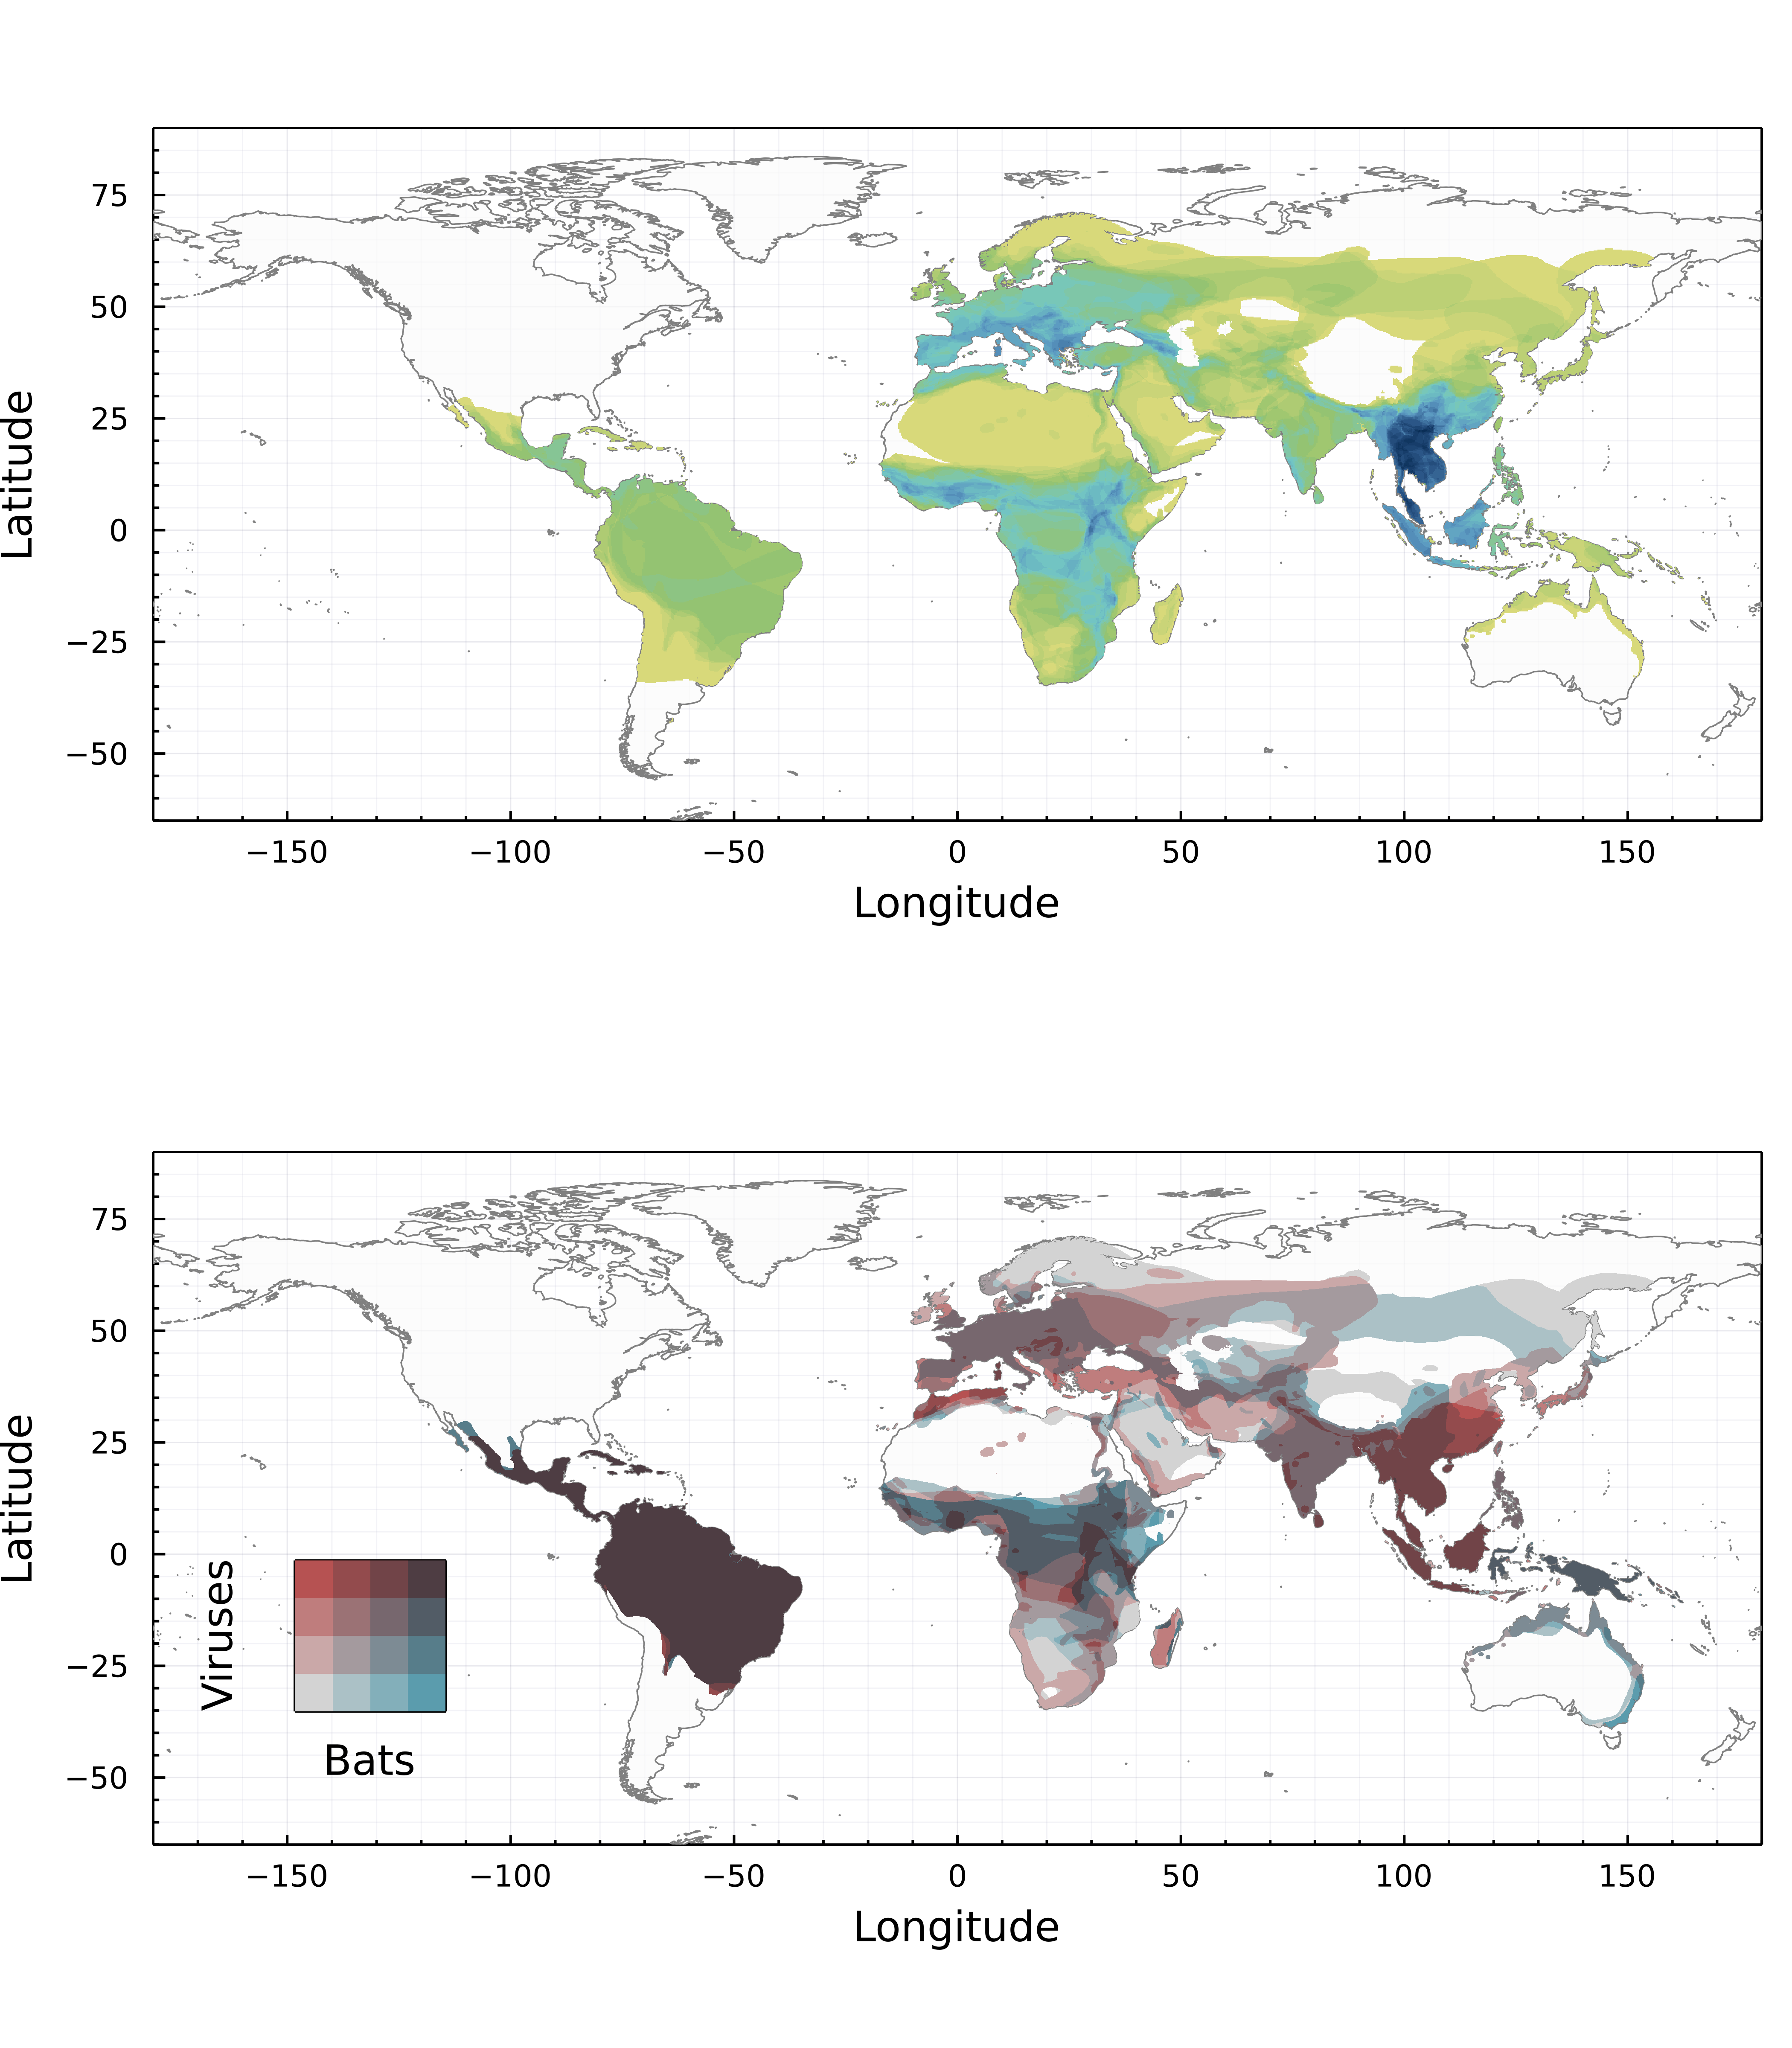
\includegraphics{figures/combined_richness.png}
\caption{Top panel: relative diversity of known bat hosts of
betacoronaviruses. This map shows that the region with the largest
number of possible hosts is South-Eastern Asia. Bottom panel: congruence
between the evolutionary distinctiveness of the hosts (grey to blue) and
the viruses (grey to red). By contrast to the richness map, this reveals
that South America has the most evolutionary distinct hosts \emph{and}
viruses, whereas South-Eastern Asia has mostly distinct viruses. This is
congruent with know results about New World bats being evolutionary
distinct, and suggests that they similarly have distinct
viruses.}\label{fig:richness}
}
\end{figure}

Nevertheless, locally diverse and virus-rich bat communities could
represent an increased risk of spillover under climate change through
the creation of novel interactions (\textbf{Ice ice berg berg}), and
therefore the diversity of betacoronavirus strains should similarly be
ccounted for. In fig.~\ref{fig:richness} (bottom), we contrast the
evolutionary distinctiveness of bats and viruses -- this reveals a
slightly different portrait than bat richness alone. Chiropterans can be
classified, from a macro-evolutionary standpoint, as microchiroptera and
macrochiroptera, where macrochiroptera have an older history from an
evolutionary perspective compared to macrochiroptera (Teeling et al.
2005, Springer 2013). Specifically, we would expect that the so-called
``New World'' group of bats, being more evolutionary distinct, would
also have evolutionary distinct viruses. Indeed fig.~\ref{fig:richness}
(bottom) reveals it to be the case, and this region harbors a distinct
bat-betacoronavirus complex. By contrast, South-Eastern Asia has a lot
of non-evolutionary distinct bats, but evolutionary-distinct viruses.

It is noteworthy that outside of South America, viral evolutionary
distinctiveness does not accurately tracks host diversity, with some
areas having over-distinct viruses (southern China but, oddly, not the
rest of southeast Asia). There are a number of likely explanations.
First, given the richness of bats in southeast Asia, many
betacoronaviruses likely remain to be discovered in this region. Indeed,
global predictions by (\textbf{Becker?}) highlight that southeast Asia
is a likely hostpot of unconfirmed hosts of betacoronaviruses, which
would likely result in additiona viral discoveries. This idea is
unsurprising given the growing realization, around the emergence of
SARS-CoV-2, that a unique lineage of similar viruses are widespread in
bats but still mostly undescribed. The most distinct
bats/betacoronavirus complex is found in South America, a region with a
comparatively lower number of hosts; this matches with the isolation
through viariance of the host group, and may highlight a different
co-evolutionary dynamic. Alternatively, this distinctiveness hostpot may
be a product of under-sampling: South-America is one of the places where
the fewest betacoronaviruses have been discovered (Anthony et al. 2017,
Olival et al. 2017, Allen et al. 2017), resulting in sparser
phylogenetic tree, thereby artificially inflating distinctiveness.
Adding more viruses would bring the distinctiveness of known sequences
down.

\hypertarget{the-phylogeographic-regions-of-hosts-and-their-viruses-overlap}{%
\subsection{The phylogeographic regions of hosts and their viruses
overlap}\label{the-phylogeographic-regions-of-hosts-and-their-viruses-overlap}}

Despite the difference in evolutionary distinctiveness globally, there
are reasons to expect that the phylogeography of bats and
betacoronaviruses should show some degree of congruence. High density of
hosts sharing the same virus (albeit possibly different strains) can
drive or result from evolution of the bat antiviral immune system,
resulting in spatially distinct immunological responses, as evidenced in
several bat species (Banerjee et al. 2020). Immune characteristics that
allow bats to be better adapted to infection by emerging viruses
(Gorbunova et al., 2020; Irving et al., 2021), in addition to being
hardcoded in their genome (\textbf{Jebb et al.~six\ldots{}}), may be
related to a wide variety of diets (Jones et al., 2022; Moreno Santillán
et al., 2021; Banerjee et al., 2020; Schneeberger et al., 2013; Muylaert
et al., 2021), themselves likely to be driven by spatial effects,
especially at the local scale -- bats, indeed, occupy a variety of
environments, and therefore display a variety of adaptations to these
environments.

\begin{figure}
\hypertarget{fig:biogeo}{%
\centering
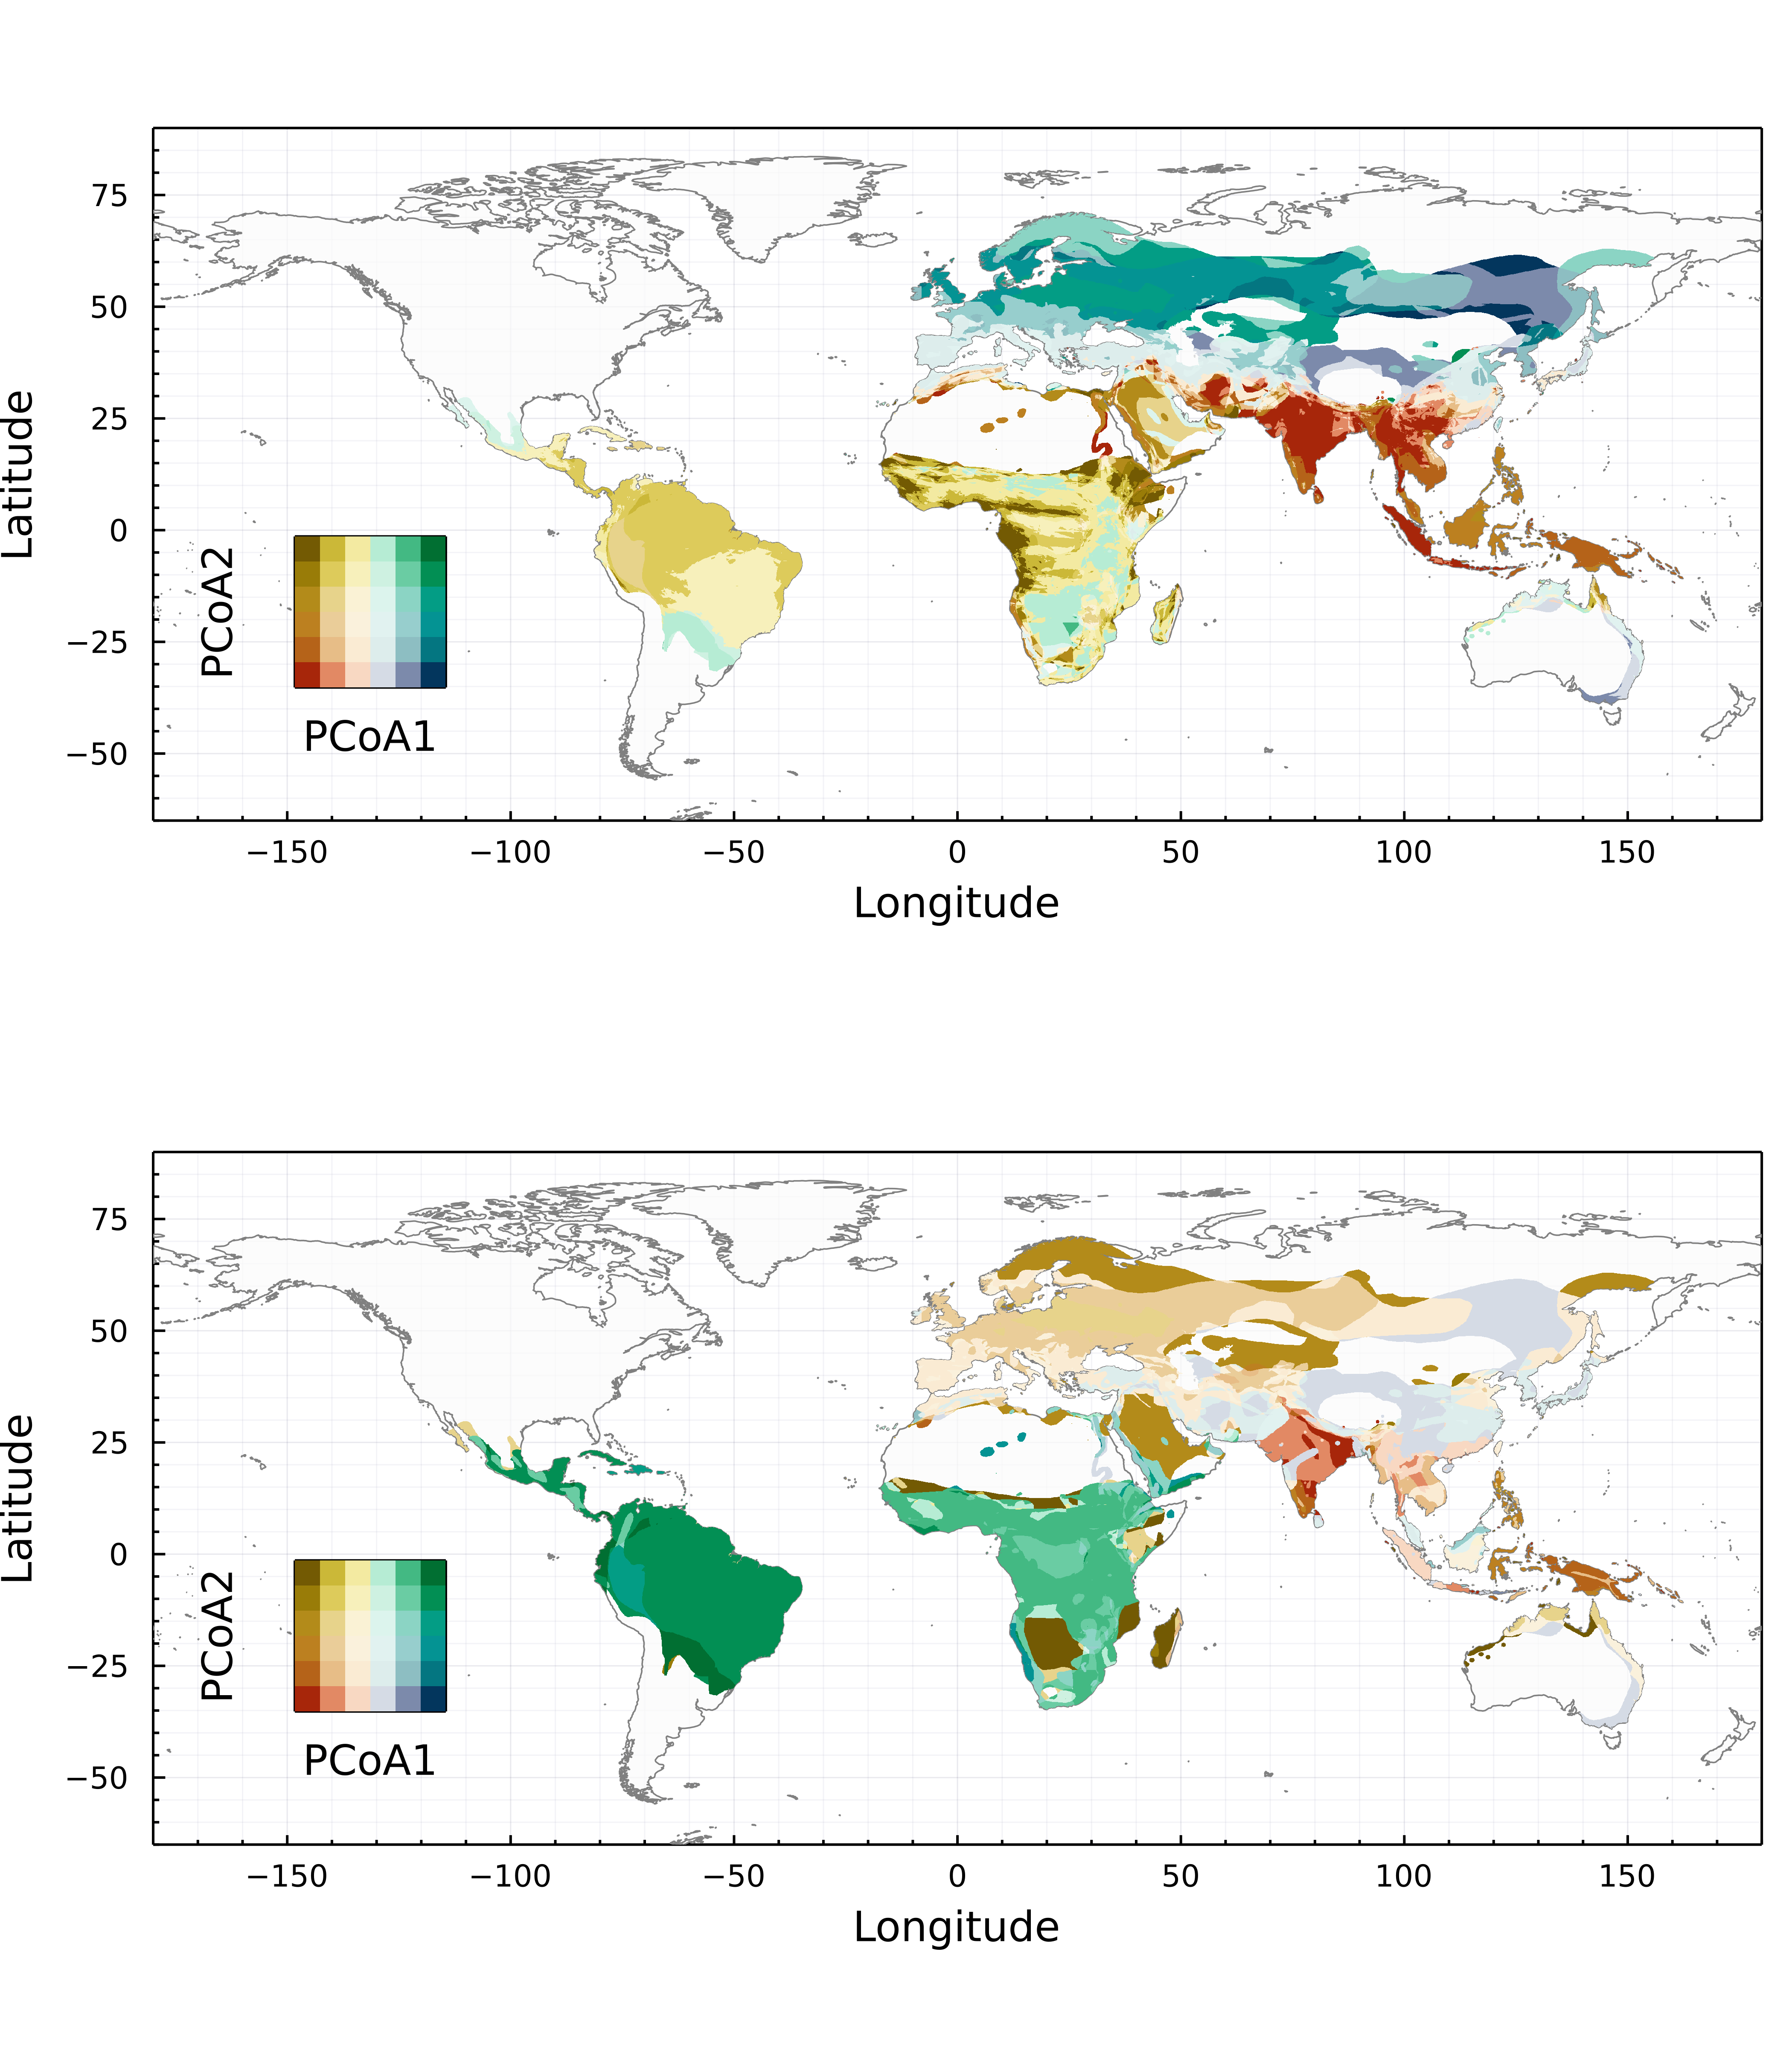
\includegraphics{figures/combined_biogeo.png}
\caption{Phylogeographic regions of bats (top) and viruses (bottom)
based on the joint analysis of their occurrence and phylogenetic
relatedness. The different colors show tendencies to separate alongside
the first two components of a PCoA. Note that the PCoA for the bats and
viruses are independent, and so cannot be compared directly -- that
being said, the regions can be compared across maps.}\label{fig:biogeo}
}
\end{figure}

In fig.~\ref{fig:biogeo}, we show a projection of the phylogeographic
signal of bats (top) and viruses (bottom) in space; the distinct
groupings (represented by different colors symbolizing positions in the
subspace formed by the first two axes of the PCoA) are essentially
equivalent between the two groups, and can be coarsely delineated as
southeast Asia, Eurasia above a northing of 25, and Africa and south
America. These results suggest that, although the evolutionary
distinctiveness of the bat/betacoronavirus complex varies spatially, the
system shows an important degree of spatial consistency, with a reduced
number of bioregions. Available information describing the spillover of
zoonotic betacoronaviruses of bat origin where data was available before
and up through the COVID-19 pandemic puts spillover events of SARS-CoV-2
in Wuhan, China; SARS-CoV in Guangdong, China based on the presence of
closest known viruses circulating in nature, and a nearby location where
serological (antibody) evidence has indicated human exposure to
SARS-like viruses (Wang et al. 2018); MERS-CoV in Saudi Arabia based on
index cases available from a recently-published compendium of cases
(Ramshaw et al. 2019). For the latest event, most if not all index cases
are presumed to be camel-to-human transmission, and the precise origin
point (if it exists) of MERS-CoV in bats is uncertain. Recent
recombinant canine coronavirus spillover events in Haiti (Lednicky et
al. 2021) and Europe (Vlasova et al. 2022) are not relevant here, as
bats' involvement in these cycles of transmission have been supposed to
be non-existent. These index cases fall within different phylogeographic
bioregions (fig.~\ref{fig:biogeo}), which further highlight the issue
that different host-virus sub-systems may lead to widespread emergence.

\hypertarget{coevolution-informed-spillover-risk-is-different-in-space}{%
\subsection{Coevolution-informed spillover risk is different in
space}\label{coevolution-informed-spillover-risk-is-different-in-space}}

As host richness, joint disctinveness, or phylogeographic structure
suggest that the bat/betacoronavirus complex is globally fragmented
enough to give rise to both different levels of risk (as evidenced by
the spatial location of spillover events) and different types of
co-evolutionary dynamics, we turn to the Geographic Mosaic Theory of
Coevolution \textbf{REF} to provide a measure of risk accounting for
multiple processes. In fig.~\ref{fig:trivariate}, we overlapped three
components of spillover risk: viral sharing, \emph{i.e.} the chance that
two bats will share viruses overall; Local Contribution to Beta
Diversity, \emph{i.e.} the fact that a bat community is compositionally
unique compared to the average compositional similarity across the
entire system; finally, host phylogenetic diversity, \emph{i.e.} how
dispersed the bats in a location are within the tree of life. This
approach leads to the definition of broad biogeographic regions of risk,
where the same color represents the same type of risk. By way of
constrat to figures fig.~\ref{fig:richness} and fig.~\ref{fig:biogeo},
these regions do not necessarilly overlap with previous spatial
partitions of the bat/betacoronavirus complex.

\begin{figure}
\hypertarget{fig:trivariate}{%
\centering
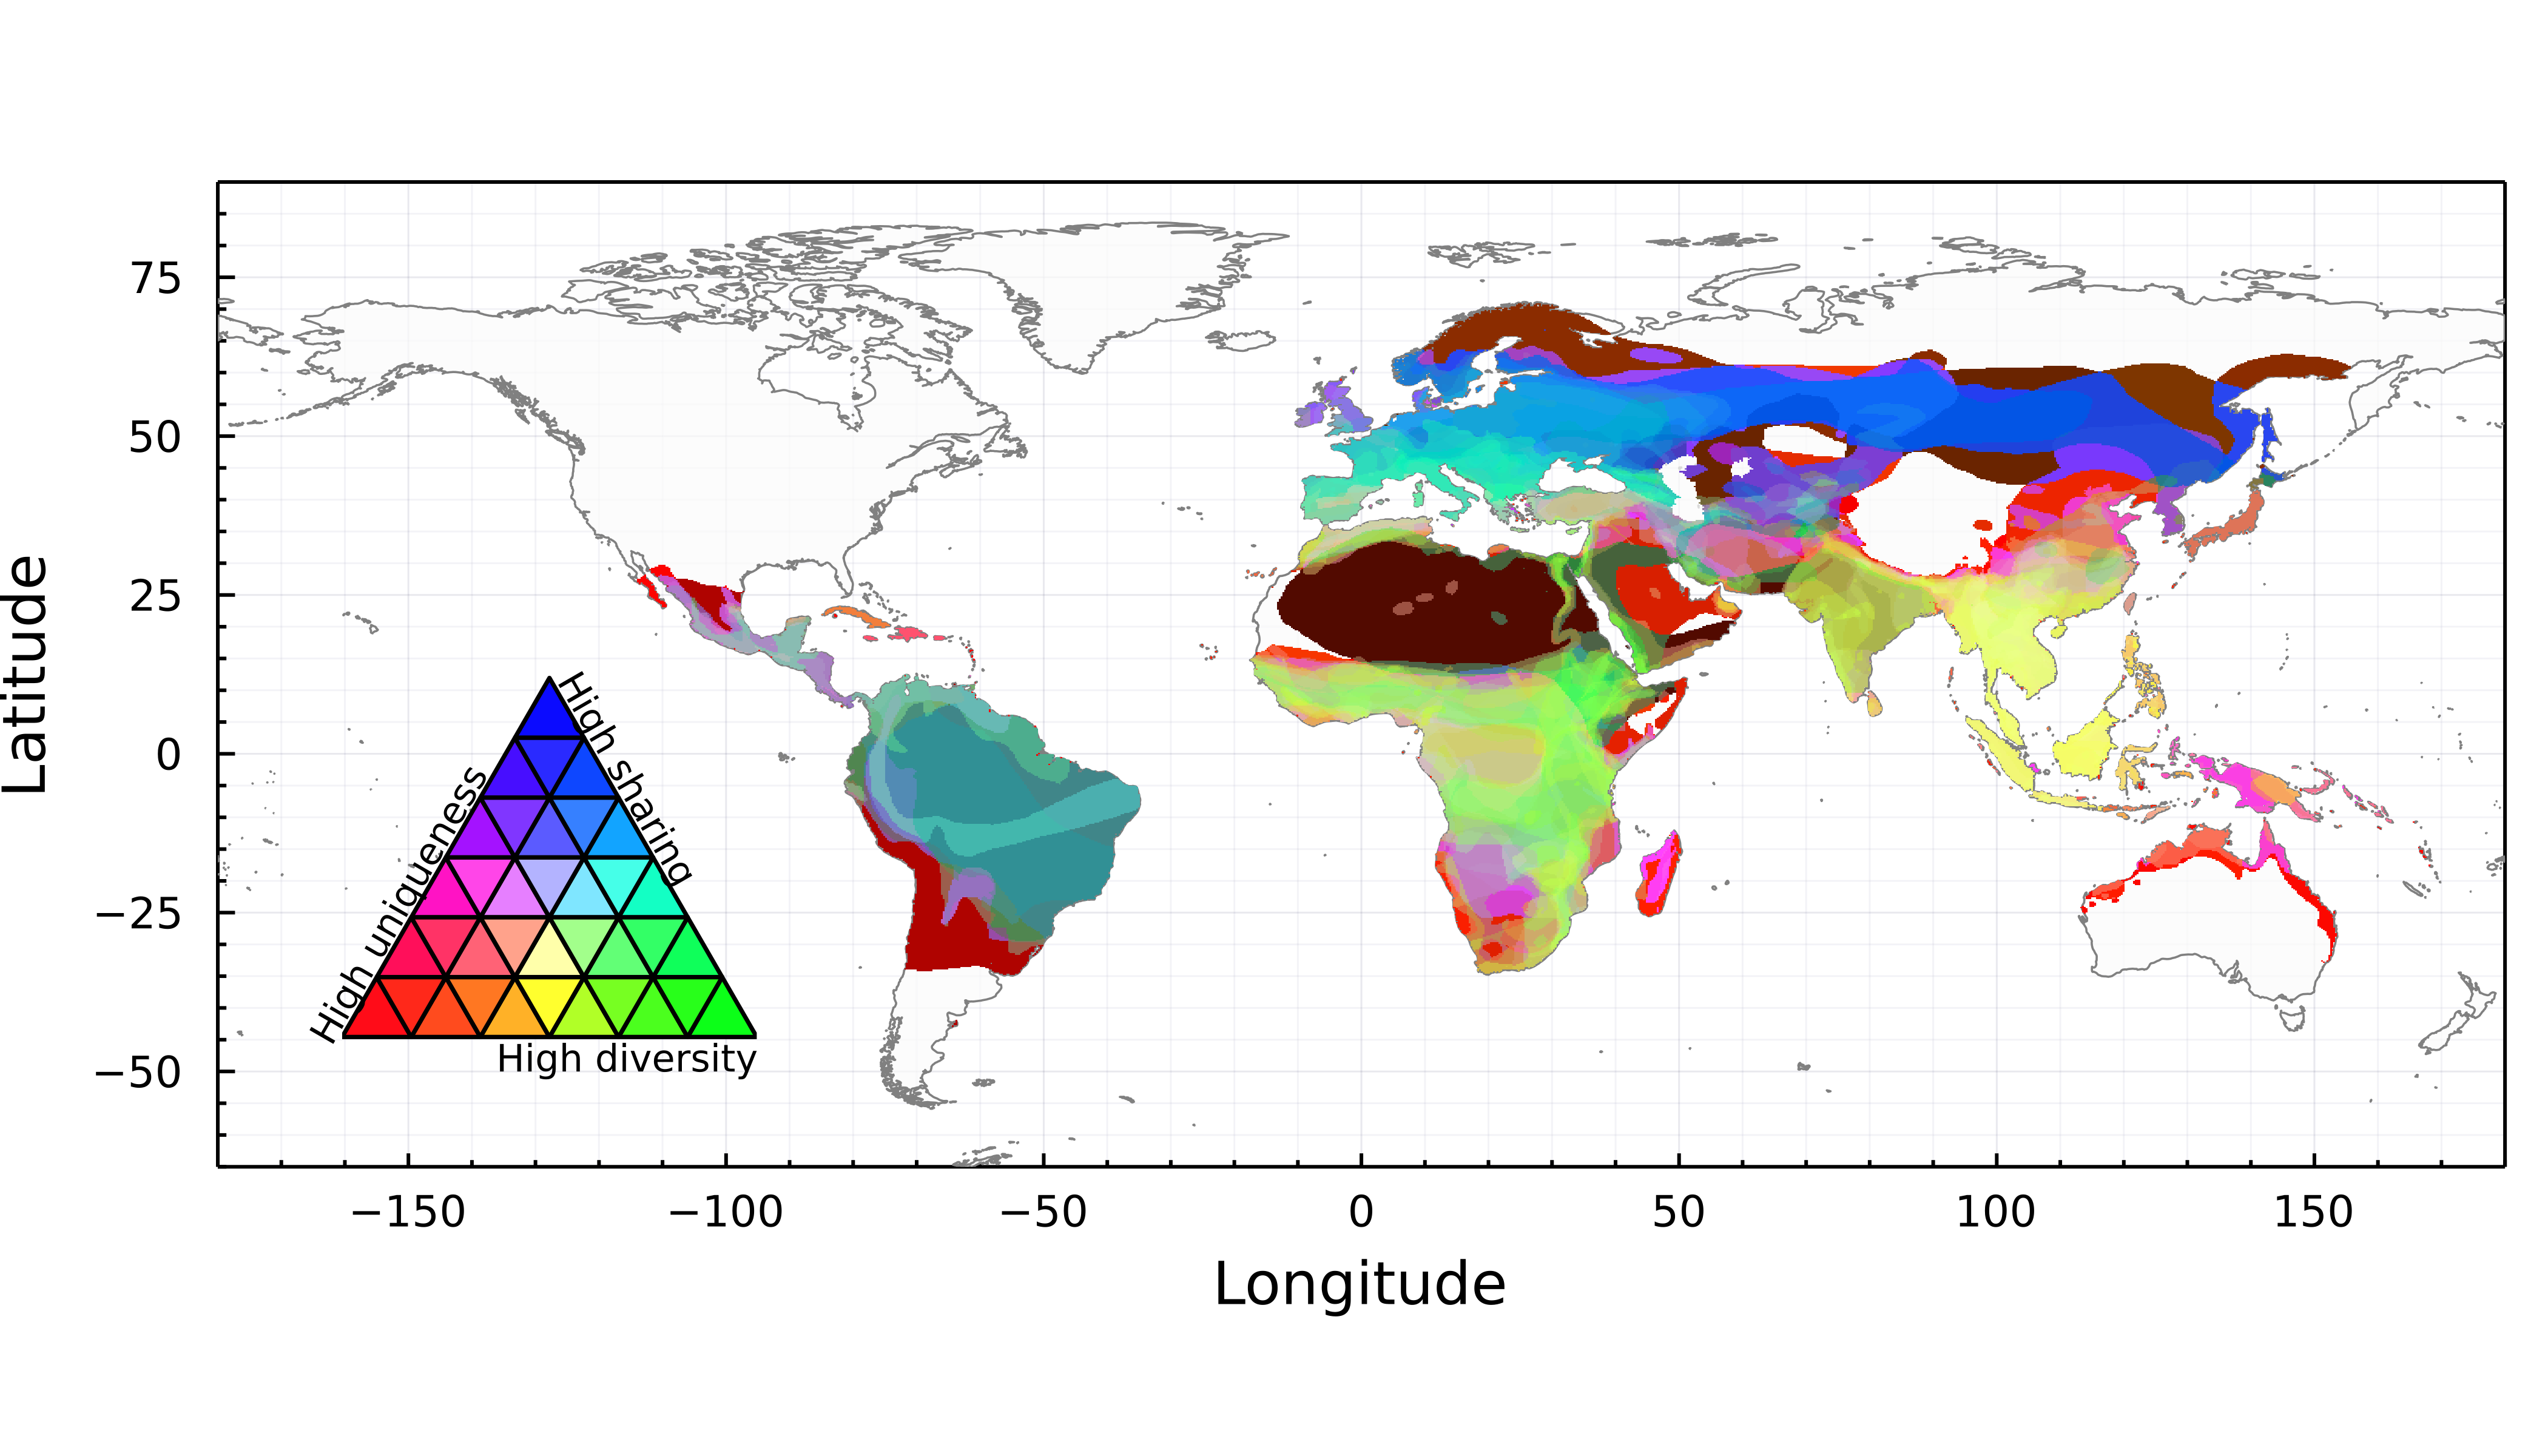
\includegraphics{figures/risk_trivariate.png}
\caption{Trivariate additive mapping of the components of risk in the
red/green/blue, where high virus sharing is encoded in the blue channel,
host phylogenetic diversity in the green channel, and compositional
uniqueness in the red channel. A pixel that would maximize all measures
would be a pure white (specifically RGB(1.0, 1.0. 1.0)), and a pixel
with the lowest possible values would be pure black (specifically
RGB(0.0, 0.0, 0.0)). Therefore, lighter values (the sum of the three
channels gets closer to 3) indicate higher risk, and the color indicates
the proportional distribution of the factors making up the total
risk.}\label{fig:trivariate}
}
\end{figure}

From the perspective of spillover risk, the most important combination
of factors is a high phylogenetic diversity of hosts with low viral
sharing; this, essentially, means that very different betacoronavirus
could co-exist within the same place. This is particularly the case
given that betacoronaviruses often evolve and even achieve host shifts
through recombination, which requires the co-occurrence of sufficiently
distinct viruses to be a major driver of emergence. In
fig.~\ref{fig:trivariate}, this corresponds to yellow to pale green
areas, which are essentially limited to South-Eastern Asia, and to some
part of Sub-Saharan Africa. Adopting a geographic mosaic theory
perspective on risk, other regions of the world are of lesser concern
fig.~\ref{fig:risk}. Our risk decomposition does not account for viral
diversity or distinctiveness. The simple rationale behind it is that the
acquisition of viral data is rarely disconnected from the acquisition of
host data; furthermore, there are more sources of information on hosts
than on viruses, allowing to develop a host-centric perspective on risk.
Areas with high bat diversity and high turnover \emph{may} facilitate
the evolutionary radiation of viruses, matching previous findings that
the diversification of bat coronaviruses is driven largely by host
shifts (inter-genus or higher levels of cross-species transmission) and,
to a lesser degree, cospeciation and sharing (intra-genus cross-species
transmission; Anthony et al. 2017). This diversification is not an
actual risk factor for spillover itself, but acts downstream of a
spillover event by increasing the random chance of the emergence of a
virus with the raw genomic components required for the potential to
infect humans.

\begin{figure}
\hypertarget{fig:risk}{%
\centering
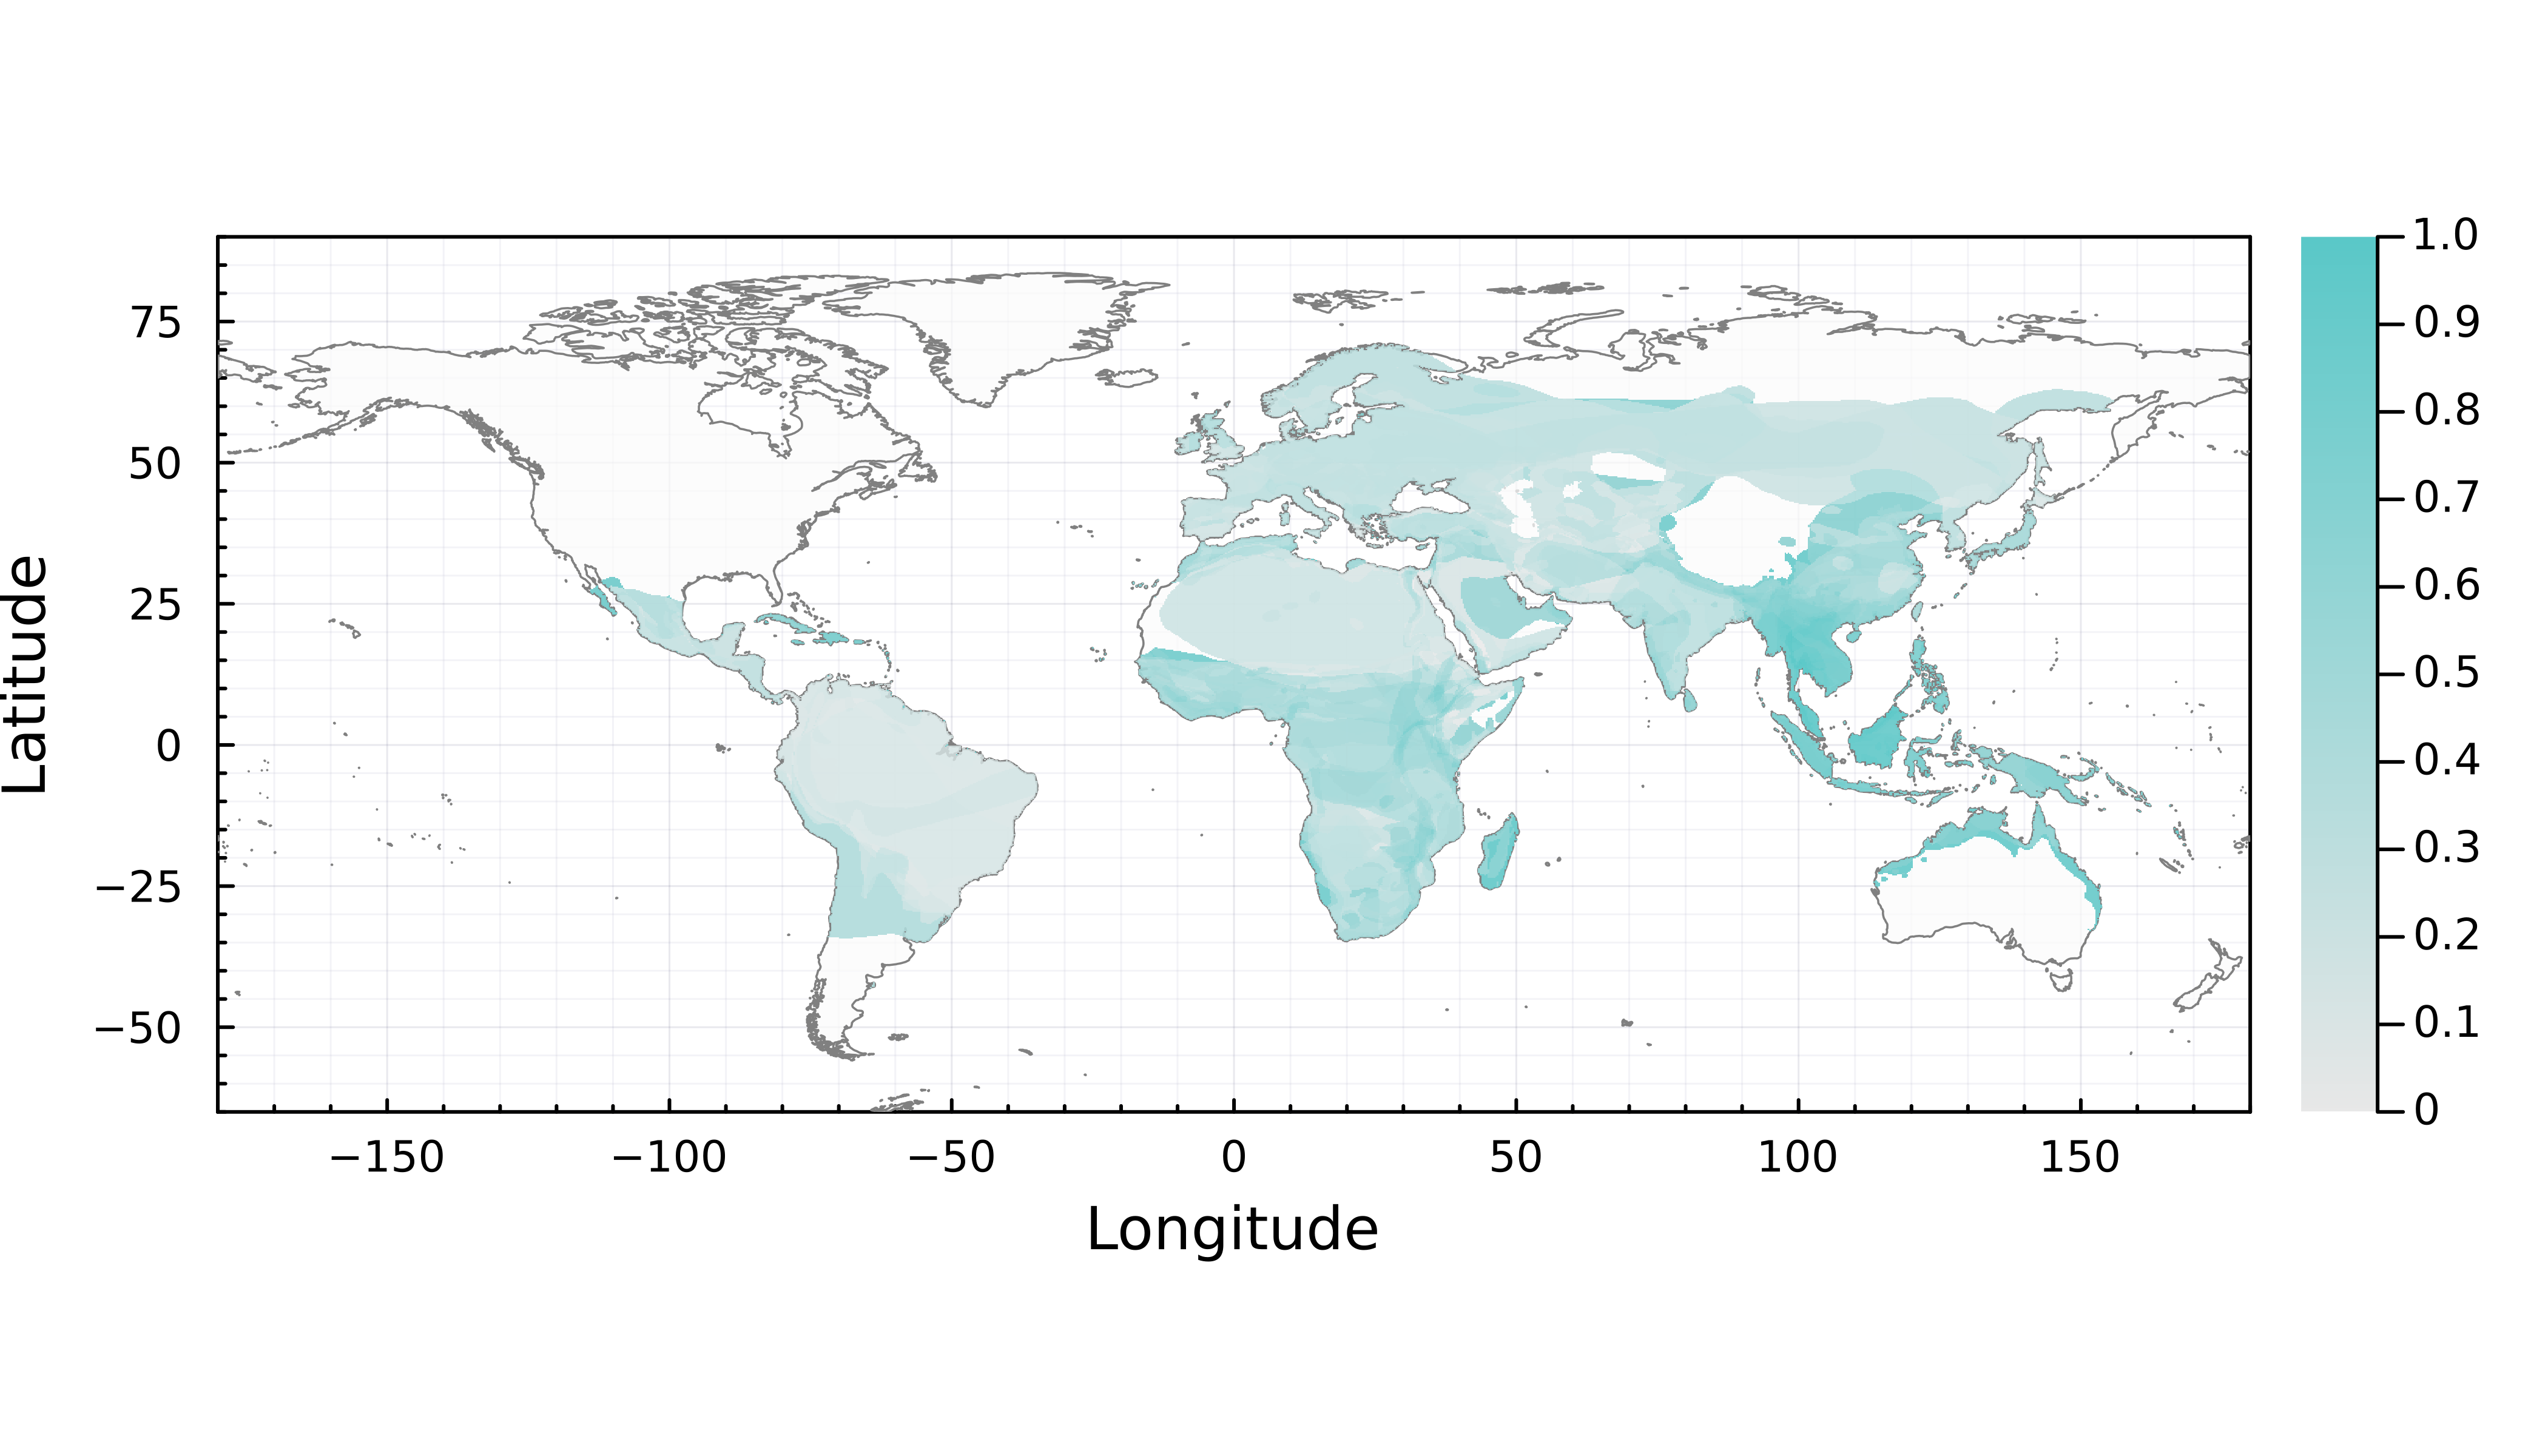
\includegraphics{figures/risk_map.png}
\caption{Extraction of a measure of risk based on the colorimetric space
from fig.~\ref{fig:trivariate}. The risk is a composite measure of the
color value and angular distance to the yellow hue, as defined in the
methods, ranged in the unit space. Based on this analyses, regions at
high risk of spillover are southeast Asia and
Madagascar.}\label{fig:risk}
}
\end{figure}

From another perspective, areas of high host uniqueness and virus
sharing (red-to-pink) could provide hotspots of betacoronavirus risk
through mixing of unique viruses (via codivergence) and in turn
recombination. Under our framework, such a hotspot was identified in
Madagascar, where most bat species are endemic following evolutionary
divergence from sister species in both African and Asian continents
(\emph{e.g.} Shi et al. 2014). Recent surveillance (Kettenburg et al.
2022) has identified a novel betacoronavirus (in the subgenus
\emph{Nobecovirus}) in Madagascar-endemic pteropid bat species
(\emph{Pteropus rufus}, \emph{Rousettus madagascariensis}), emphasizing
strong proof of principle in model predictions.

\hypertarget{human-occupancy-drives-different-levels-of-effective-risk-globally}{%
\subsection{Human occupancy drives different levels of effective risk
globally}\label{human-occupancy-drives-different-levels-of-effective-risk-globally}}

Based on the previous result, we extracted the risk component from the
composite map (see Methods), to provide a single measure of risk varying
between 0 and 1. This measure is presented in fig.~\ref{fig:risk}.
However, this maps the potential risk, which must be weighed by the
potential for contacts with humans. As a proxy for this measure, we used
the proportion of build/urban land from the EarthEnv dataset: this is a
reasonable proxy for the density of humans per unit area, which
increases the probability of pathogen spread more widely (Hazarie et al.
2021). Since human activity is required to amplify the frequency of
virus encounters and thus create areas of viral amplification, mapping
the potential risk against measures of land use is required to generate
a more actionable assessment of risk. This map is presented in
fig.~\ref{fig:compound}. Most of South America and Europe are at low
risk, as although densely populated, settlements tend to be in areas
with lower potential risk. However, this mapping reveals that South-East
Asia, the Indian subcontinent, and parts of sub-Saharan Africa, are at
high risk due to the overlap between built areas and bat communities
representing more opportunities for cross-species transmission of
betacoronaviruses. In looking for the origins of SARS in China, Xu et
al. (2004) present serological evidence that strongest human-animal
contact results in higher risk of virus exposure, regardless of the
animal species, but that different types of contact had different
impacts. Ideally, finer-grained information about human activity (rather
than human presence through anthropisation) could allow to partition
this risk further.

\begin{figure}
\hypertarget{fig:compound}{%
\centering
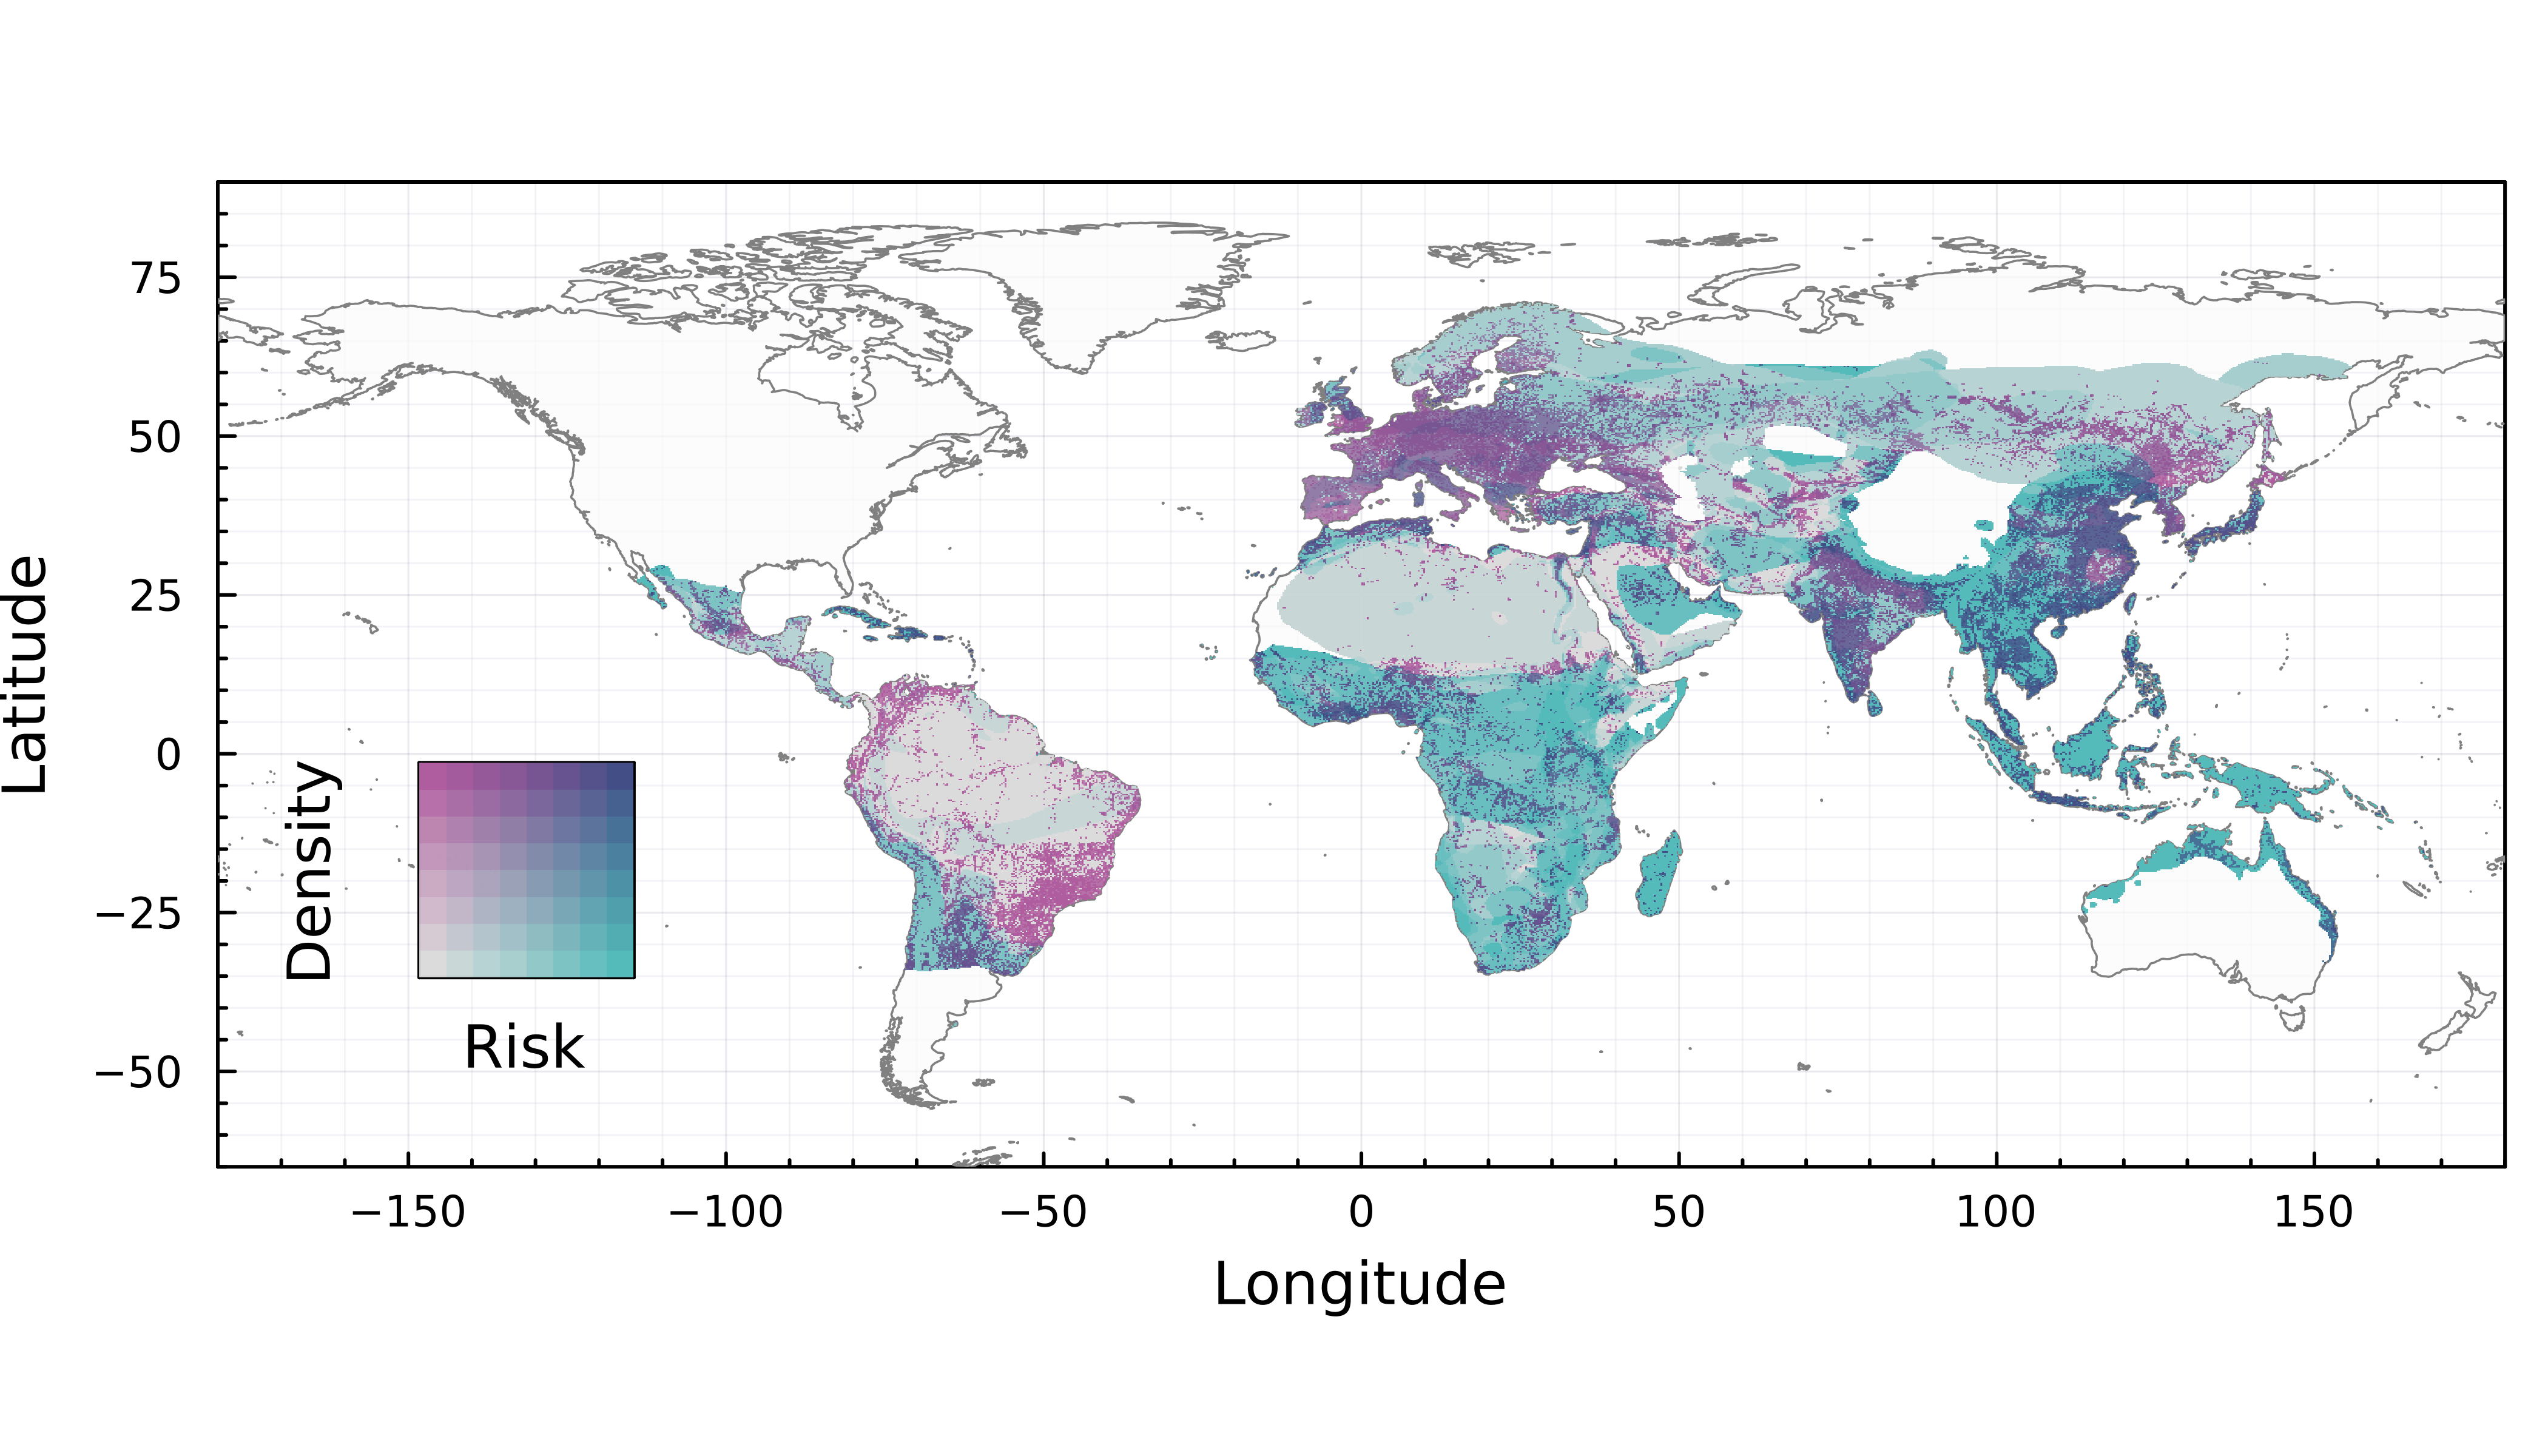
\includegraphics{figures/risk_compounded.png}
\caption{Overlap of the percent of each pixel occupied by urbanized
structures, representing the degree of settlement, on the risk map.
Darker pixels correspond to more risk, in that the GMTC-derived risk of
fig.~\ref{fig:risk} is high \emph{and} the pixel is densely occupied by
human populations. This approach increases the relative risk of several
regions in Africa, and highlights the risk in India, southeast China,
and the arabic peninsula where areas of high to moderate risk overlap
with areas of denser population.}\label{fig:compound}
}
\end{figure}

\hypertarget{conclusion}{%
\section{Conclusion}\label{conclusion}}

Our study focuses largely on the biogeography of hosts. Yet, we know
that viruses with high host plasticity, that is, the ability of a given
virus to adapt to various taxonomic orders and ecological groups
(Kreuder Johnson et al. 2015), are more likely to amplify viral
spillover, followed by secondary human-to-human transmission, and
geographical spread (Hazarie et al. 2021). High viral host plasticity is
an especially important trait for RNA viruses like betacoronaviruses
(Haddad et al. 2021). Indeed, our analysis of viral sequences reveals
that Latin America is a hotspot of viral distinctiveness, suggesting
that this part of the bats-betacoronavirus system may be undergoing
independent evolutionary dynamics (related species sharing viruses that
are different from the rest of the global pool). The other hotspot of
viral distinctiveness is S.E. Asia, in which richness is high but
sharing is low; this suggests a different type of evolutionary dynamics
(unrelated viruses coevolving with evolutionarily distinct hosts,
generating high diversity locally). Both of these areas should be
priority areas for sampling, especially since Becker et al. (2022)
advance that they harbor undiscovered hosts of beta-coronaviruses. This
diversity of hosts, and the mechanisms by which the exchange of viruses
occurs between species, is largely affected by the local environmental
conditions and environmental change.

Bats are important reservoir hosts for different classes of
microorganisms, many of which a threat to human health (Letko et al.
2020, Van Brussel and Holmes 2022). Chiropterans emerged around 64
million years ago and are one of the most diverse mammalian orders, with
an estimated richness of more than 1400 species (Peixoto et al. 2018,
Simmons and Cirranello 2020). They exhibit a broad variety of habitat
use, behaviour, and feeding strategies, putting them at key positions in
the delivery and provisioning of several ecosystem services, tied to
important ecosystem-derived benefits to human (Kasso and Balakrishnan
2013). For example, bats are an essential component of many
seed-dispersal networks (Mello et al. 2011). Over two-thirds of bats are
know to be either obligate or facultative insectivores, therefore
playing an important role in the regulation of insect pests that can
affect crops (Williams-Guillén et al. 2008, Voigt and Kingston 2016),
and vectors of pathogens that put a risk on human health (Gonsalves et
al. 2013a, b). Because bats are globally distributed and have a long
evolutionary history, phylogeographic and biogeographic approaches are
required to shed light on the contemporary distribution of
coevolutionary processes between bats and the pathogens they host. Not
all areas in which bats, viruses, and human are co-occuring are facing a
risk of spillover towards human populations, and the areas in which this
risk exist may not be facing risks of the same nature and magnitude.

There are several factors that drive changes in the diversity of bats
(Alves et al. 2018), but human activities' effects on the ecosystem
(like modifications of land use) could significantly decrease it.
Therefore, it can be suggested that changes in the diversity of betacovs
in bats are linked to their biogeographic variation, and human
population density and other anthropogenic factors are decisive
moderators for its implications in public health. With the increase of
contact between humans and potential hosts, we also increase the risk of
emergence of novel diseases (Johnson et al. 2020), as previous studies
on RNA viruses suggest the importance of host phylogeography at the time
of virus dispersal (Gryseels et al. 2017). One of these scenarios where
interaction between bats and humans can occur can be seed dispersal in
tropical agroecosystems. It opens the discussion of whether the fruits
thrown by bats not only disperse seeds but could also be a source of
indirect interaction between viruses of bat origin and humans (Deshpande
et al. 2022). This represents a challenge for conservation strategies
and disease ecology since some areas can haveboth potential for the
acquisition of zoonotic viruses and bat-human interactions; in
particular, the challenge lies in the fact that actual exposure must
then be quantified accounting for several transmission scenarios,
including both direct and indirect bat - human interaction.

\textbf{Acknowledgements}: We acknowledge that this study was conducted
on land within the traditional unceded territory of the Saint Lawrence
Iroquoian, Anishinabewaki, Mohawk, Huron-Wendat, and Omàmiwininiwak
nations. This work was supported by funding to the Viral Emergence
Research Initiative (VERENA) consortium including NSF BII 2021909 and a
grant from Institut de Valorisation des Données (IVADO). This research
was enabled in part by support provided by Calcul Québec
(www.calculquebec.ca) and Compute Canada (www.computecanada.ca). NF is
funded by the NSERC BIOS² CREATE program. TP and NF are funded by the
Courtois Foundation. RLM was supported by Bryce Carmine and Anne Carmine
(née Percival), through the Massey University Foundation.

\hypertarget{references}{%
\section*{References}\label{references}}
\addcontentsline{toc}{section}{References}

\hypertarget{refs}{}
\begin{CSLReferences}{1}{0}
\leavevmode\hypertarget{ref-Agosta2010HowSpe}{}%
Agosta, S. J. et al. 2010. How specialists can be generalists: Resolving
the {``parasite paradox''} and implications for emerging infectious
disease. - Zoologia (Curitiba) 27: 151--162.

\leavevmode\hypertarget{ref-Albery2020PreGlo}{}%
Albery, G. F. et al. 2020. Predicting the global mammalian viral sharing
network using phylogeography. - Nature Communications 11: 2260.

\leavevmode\hypertarget{ref-Albery2022UrbMam}{}%
Albery, G. F. et al. 2022. Urban-adapted mammal species have more known
pathogens. in press.

\leavevmode\hypertarget{ref-Allen2017GloHot}{}%
Allen, T. et al. 2017. Global hotspots and correlates of emerging
zoonotic diseases. - Nature Communications in press.

\leavevmode\hypertarget{ref-Alves2018GeoVar}{}%
Alves, D. M. C. C. et al. 2018. Geographic variation in the relationship
between large-scale environmental determinants and bat species richness.
- Basic and Applied Ecology 27: 1--8.

\leavevmode\hypertarget{ref-Anthony2017GloPat}{}%
Anthony, S. J. et al. 2017. Global patterns in coronavirus diversity. -
Virus Evolution in press.

\leavevmode\hypertarget{ref-Banerjee2020NovIns}{}%
Banerjee, A. et al. 2020. Novel Insights Into Immune Systems of Bats. -
Frontiers in Immunology 11: 26.

\leavevmode\hypertarget{ref-Becker2020InfInt}{}%
Becker, D. J. et al. 2020. Beyond Infection: Integrating Competence into
Reservoir Host Prediction. - Trends in Ecology \& Evolution 35:
1062--1065.

\leavevmode\hypertarget{ref-Becker2022OptPre}{}%
Becker, D. J. et al. 2022. Optimising predictive models to prioritise
viral discovery in zoonotic reservoirs. - The Lancet Microbe in press.

\leavevmode\hypertarget{ref-Calisher2006BatImp}{}%
Calisher, C. H. et al. 2006. Bats: Important Reservoir Hosts of Emerging
Viruses. - Clinical Microbiology Reviews 19: 531--545.

\leavevmode\hypertarget{ref-Cavender-Bares2009MerCom}{}%
Cavender-Bares, J. et al. 2009. The merging of community ecology and
phylogenetic biology. - Ecol. Lett. 12: 693--715.

\leavevmode\hypertarget{ref-Dansereau2022EvaEco}{}%
Dansereau, G. et al. 2022. Evaluating ecological uniqueness over broad
spatial extents using species distribution modelling. - Oikos n/a:
e09063.

\leavevmode\hypertarget{ref-Deshpande2022ForFru}{}%
Deshpande, K. et al. 2022. Forbidden fruits? Ecosystem services from
seed dispersal by fruit bats in the context of latent zoonotic risk. -
Oikos (Copenhagen, Denmark): oik.08359.

\leavevmode\hypertarget{ref-Drexler2014EcoEvo}{}%
Drexler, J. F. et al. 2014. Ecology, evolution and classification of bat
coronaviruses in the aftermath of SARS. - Antiviral Research 101:
45--56.

\leavevmode\hypertarget{ref-Engering2013PatHos}{}%
Engering, A. et al. 2013. Pathogen--host--environment interplay and
disease emergence. - Emerging Microbes \& Infections 2: e5.

\leavevmode\hypertarget{ref-Faith1992ConEva}{}%
Faith, D. P. 1992. Conservation evaluation and phylogenetic diversity. -
Biological Conservation 61: 1--10.

\leavevmode\hypertarget{ref-Gomulkiewicz2000HotSpo}{}%
Gomulkiewicz, R. et al. 2000. Hot Spots, Cold Spots, and the Geographic
Mosaic Theory of Coevolution. - The American Naturalist 156: 156--174.

\leavevmode\hypertarget{ref-Gonsalves2013MosInf}{}%
Gonsalves, L. et al. 2013a. Do mosquitoes influence bat activity in
coastal habitats? - Wildlife Research 40: 10--24.

\leavevmode\hypertarget{ref-Gonsalves2013MosCon}{}%
Gonsalves, L. et al. 2013b. Mosquito Consumption by Insectivorous Bats:
Does Size Matter? - PLOS ONE 8: e77183.

\leavevmode\hypertarget{ref-Gryseels2017WheVir}{}%
Gryseels, S. et al. 2017. When Viruses Don't Go Viral: The Importance of
Host Phylogeographic Structure in the Spatial Spread of Arenaviruses (JH
Kuhn, Ed.). - PLOS Pathogens 13: e1006073.

\leavevmode\hypertarget{ref-Haddad2021SarPos}{}%
Haddad, D. et al. 2021. SARS-CoV-2: Possible recombination and emergence
of potentially more virulent strains (H Attoui, Ed.). - PLOS ONE 16:
e0251368.

\leavevmode\hypertarget{ref-Hazarie2021IntPop}{}%
Hazarie, S. et al. 2021. Interplay between population density and
mobility in determining the spread of epidemics in cities. -
Communications Physics 4: 191.

\leavevmode\hypertarget{ref-Isaac2007MamEdg}{}%
Isaac, N. J. B. et al. 2007. Mammals on the EDGE: Conservation
Priorities Based on Threat and Phylogeny. - PLOS ONE 2: e296.

\leavevmode\hypertarget{ref-IUCN2021IucRed}{}%
IUCN 2021. The IUCN Red List of Threatened Species.

\leavevmode\hypertarget{ref-Johnson2020GloShi}{}%
Johnson, C. K. et al. 2020. Global shifts in mammalian population trends
reveal key predictors of virus spillover risk. - Proceedings of the
Royal Society B: Biological Sciences 287: 20192736.

\leavevmode\hypertarget{ref-Kasso2013EcoEco}{}%
Kasso, M. and Balakrishnan, M. 2013. Ecological and Economic Importance
of Bats (Order Chiroptera). - ISRN Biodiversity 2013: e187415.

\leavevmode\hypertarget{ref-Keke2010StuSki}{}%
Keke, S. et al. 2010. Study on skin color image segmentation used by
Fuzzy-c-means arithmetic. - 2010 Seventh International Conference on
Fuzzy Systems and Knowledge Discovery 2: 612--615.

\leavevmode\hypertarget{ref-Kettenburg2022FulGen}{}%
Kettenburg, G. et al. 2022. Full Genome Nobecovirus Sequences From
Malagasy Fruit Bats Define a Unique Evolutionary History for This
Coronavirus Clade. - Frontiers in Public Health in press.

\leavevmode\hypertarget{ref-Kreft2007GloPat}{}%
Kreft, H. and Jetz, W. 2007. Global patterns and determinants of
vascular plant diversity. - Proceedings of the National Academy of
Sciences 104: 5925--5930.

\leavevmode\hypertarget{ref-Kreft2010FraDel}{}%
Kreft, H. and Jetz, W. 2010. A framework for delineating biogeographical
regions based on species distributions. - Journal of Biogeography 37:
2029--2053.

\leavevmode\hypertarget{ref-KreuderJohnson2015SpiPan}{}%
Kreuder Johnson, C. et al. 2015. Spillover and pandemic properties of
zoonotic viruses with high host plasticity. - Scientific Reports 5:
14830.

\leavevmode\hypertarget{ref-Lednicky2021IsoNov}{}%
Lednicky, J. A. et al. 2021. Isolation of a Novel Recombinant Canine
Coronavirus from a Visitor to Haiti: Further Evidence of Transmission of
Coronaviruses of Zoonotic Origin to Humans. - Clinical Infectious
Diseases: An Official Publication of the Infectious Diseases Society of
America: ciab924.

\leavevmode\hypertarget{ref-Legendre2013BetDiv}{}%
Legendre, P. and De Cáceres, M. 2013. Beta diversity as the variance of
community data: Dissimilarity coefficients and partitioning (H Morlon,
Ed.). - Ecology Letters 16: 951--963.

\leavevmode\hypertarget{ref-Legendre2019SpaTem}{}%
Legendre, P. and Condit, R. 2019. Spatial and temporal analysis of beta
diversity in the Barro Colorado Island forest dynamics plot, Panama. -
Forest Ecosystems 6: 7.

\leavevmode\hypertarget{ref-Letko2020BatVir}{}%
Letko, M. et al. 2020. Bat-borne virus diversity, spillover and
emergence. - Nature Reviews Microbiology 18: 461--471.

\leavevmode\hypertarget{ref-MacLean2021NatSel}{}%
MacLean, O. A. et al. 2021. Natural selection in the evolution of
SARS-CoV-2 in bats created a generalist virus and highly capable human
pathogen. - PLOS Biology 19: e3001115.

\leavevmode\hypertarget{ref-Melaun2014BatPot}{}%
Melaun, C. et al. 2014. Bats as Potential Reservoir Hosts for
Vector-Borne Diseases. - In: Klimpel, S. and Mehlhorn, H. (eds), Bats
(Chiroptera) as Vectors of Diseases and Parasites: Facts and Myths.
Parasitology Research Monographs. Springer, pp. 25--61.

\leavevmode\hypertarget{ref-Mello2011MisPar}{}%
Mello, M. A. R. et al. 2011. The Missing Part of Seed Dispersal
Networks: Structure and Robustness of Bat-Fruit Interactions. - PLOS ONE
6: e17395.

\leavevmode\hypertarget{ref-Mollentze2020VirZoo}{}%
Mollentze, N. and Streicker, D. G. 2020. Viral zoonotic risk is
homogenous among taxonomic orders of mammalian and avian reservoir
hosts. - Proceedings of the National Academy of Sciences 117:
9423--9430.

\leavevmode\hypertarget{ref-Moratelli2015BatZoo}{}%
Moratelli, R. and Calisher, C. H. 2015. Bats and zoonotic viruses: Can
we confidently link bats with emerging deadly viruses? - Memórias do
Instituto Oswaldo Cruz 110: 1--22.

\leavevmode\hypertarget{ref-Mull2022VirIso}{}%
Mull, N. et al. 2022. Virus isolation data improve host predictions for
New World rodent orthohantaviruses. - Journal of Animal Ecology in
press.

\leavevmode\hypertarget{ref-Olival2017HosVir}{}%
Olival, K. J. et al. 2017. Host and viral traits predict zoonotic
spillover from mammals. - Nature 546: 646--650.

\leavevmode\hypertarget{ref-Paradis2019ApeEnv}{}%
Paradis, E. and Schliep, K. 2019. Ape 5.0: An environment for modern
phylogenetics and evolutionary analyses in R. - Bioinformatics 35:
526--528.

\leavevmode\hypertarget{ref-Peixoto2018SynEco}{}%
Peixoto, F. P. et al. 2018. A synthesis of ecological and evolutionary
determinants of bat diversity across spatial scales. - BMC ecology 18:
18.

\leavevmode\hypertarget{ref-Plowright2015EcoDyn}{}%
Plowright, R. K. et al. 2015. Ecological dynamics of emerging bat virus
spillover. - Proceedings of the Royal Society B: Biological Sciences
282: 20142124.

\leavevmode\hypertarget{ref-Plowright2017PatZoo}{}%
Plowright, R. K. et al. 2017. Pathways to zoonotic spillover. - Nature
Reviews Microbiology 15: 502--510.

\leavevmode\hypertarget{ref-Power2004PatSpi}{}%
Power, A. G. and Mitchell, C. E. 2004. Pathogen Spillover in Disease
Epidemics. - The American Naturalist 164: S79--S89.

\leavevmode\hypertarget{ref-Ramshaw2019DatGeo}{}%
Ramshaw, R. E. et al. 2019. A database of geopositioned Middle East
Respiratory Syndrome Coronavirus occurrences. - Scientific Data 6: 318.

\leavevmode\hypertarget{ref-Rego2015AssHum}{}%
Rego, K. M. da C. et al. 2015. Assessing human-bat interactions around a
protected area in northeastern Brazil. - Journal of Ethnobiology and
Ethnomedicine 11: 80.

\leavevmode\hypertarget{ref-RouaultEven2022GdaOgr}{}%
Rouault, E. et al. 2022. GDAL/OGR Geospatial Data Abstraction software
Library. - Zenodo.

\leavevmode\hypertarget{ref-Seekell2018GeoLak}{}%
Seekell, D. A. et al. 2018. A geography of lake carbon cycling. -
Limnology and Oceanography Letters 3: 49--56.

\leavevmode\hypertarget{ref-Shi2014DeeDiv}{}%
Shi, J. J. et al. 2014. A Deep Divergence Time between Sister Species of
Eidolon (Pteropodidae) with Evidence for Widespread Panmixia. - Acta
Chiropterologica 16: 279--292.

\leavevmode\hypertarget{ref-Simmons2020BatSpe}{}%
Simmons, N. B. and Cirranello, A. L. 2020. Bat Species of the World: A
taxonomic and geographic database.

\leavevmode\hypertarget{ref-Springer2013PhyBat}{}%
Springer, M. S. 2013. Phylogenetics: Bats United, Microbats Divided. -
Current Biology 23: R999--R1001.

\leavevmode\hypertarget{ref-Stone2015ManCon}{}%
Stone, E. et al. 2015. Managing Conflict between Bats and Humans: The
Response of Soprano Pipistrelles (Pipistrellus pygmaeus) to Exclusion
from Roosts in Houses. - PLoS ONE 10: e0131825.

\leavevmode\hypertarget{ref-Teeling2005MolPhy}{}%
Teeling, E. C. et al. 2005. A Molecular Phylogeny for Bats Illuminates
Biogeography and the Fossil Record. - Science (New York, N.Y.) 307:
580--584.

\leavevmode\hypertarget{ref-Thompson2005GeoMos}{}%
Thompson, J. N. 2005. The Geographic Mosaic of Coevolution. - University
Of Chicago Press.

\leavevmode\hypertarget{ref-Upham2019InfMam}{}%
Upham, N. S. et al. 2019. Inferring the mammal tree: Species-level sets
of phylogenies for questions in ecology, evolution, and conservation. -
PLOS Biology 17: e3000494.

\leavevmode\hypertarget{ref-VanBrussel2022ZooDis}{}%
Van Brussel, K. and Holmes, E. C. 2022. Zoonotic disease and virome
diversity in bats. - Current Opinion in Virology 52: 192--202.

\leavevmode\hypertarget{ref-Vlasova2022AniAlp}{}%
Vlasova, A. N. et al. 2022. Animal alphacoronaviruses found in human
patients with acute respiratory illness in different countries. -
Emerging Microbes \& Infections 11: 699--702.

\leavevmode\hypertarget{ref-Voigt2016BatAnt}{}%
2016. Bats in the Anthropocene: Conservation of Bats in a Changing World
(CC Voigt and T Kingston, Eds.). - Springer International Publishing.

\leavevmode\hypertarget{ref-Wang2018SerEvi}{}%
Wang, N. et al. 2018. Serological Evidence of Bat SARS-Related
Coronavirus Infection in Humans, China. - Virologica Sinica 33:
104--107.

\leavevmode\hypertarget{ref-Williams-Guillen2008BatLim}{}%
Williams-Guillén, K. et al. 2008. Bats Limit Insects in a Neotropical
Agroforestry System. - Science 320: 70--70.

\leavevmode\hypertarget{ref-Xu2004EpiClu}{}%
Xu, R.-H. et al. 2004. Epidemiologic Clues to SARS Origin in China. -
Emerging Infectious Diseases 10: 1030--1037.

\end{CSLReferences}

\end{document}
